\documentclass[11pt]{article}
\usepackage[T1]{fontenc}
\usepackage[utf8]{inputenc}
\usepackage{lmodern}
\usepackage{amsmath,amssymb,amsthm,mathtools}
\usepackage{mathrsfs}
\usepackage{microtype}
\usepackage[margin=1.05in]{geometry}
\usepackage{enumitem}
\usepackage{tikz}
\usetikzlibrary{arrows.meta,positioning,calc}
\usepackage{xcolor}
\usepackage{hyperref}
\hypersetup{colorlinks=true,linkcolor=blue!45!black,citecolor=blue!45!black,
  urlcolor=blue!45!black,pdftitle={Numerical semiampleness of nef adjoint classes on compact Kahler manifolds},
  pdfauthor={OpenAI}}
\newcommand{\Q}{\mathbb Q}
\newcommand{\R}{\mathbb R}
\newcommand{\C}{\mathbb C}
\newcommand{\Z}{\mathbb Z}
\newcommand{\N}{\mathbb N}
\newcommand{\PP}{\mathbb P}
\newcommand{\cO}{\mathcal O}
\newcommand{\num}{\equiv}
\newcommand{\qsim}{\sim_{\Q}}
\DeclareMathOperator{\Pic}{Pic}
\DeclareMathOperator{\Supp}{Supp}
\DeclareMathOperator{\codim}{codim}
\DeclareMathOperator{\rank}{rank}
\DeclareMathOperator{\vol}{vol}
\DeclareMathOperator{\im}{im}
\DeclareMathOperator{\tr}{tr}
\DeclareMathOperator{\Alb}{Alb}
\newtheorem{theorem}{Theorem}[section]
\newtheorem{proposition}[theorem]{Proposition}
\newtheorem{lemma}[theorem]{Lemma}
\newtheorem{corollary}[theorem]{Corollary}
\newtheorem{claim}[theorem]{Claim}
\theoremstyle{definition}
\newtheorem{definition}[theorem]{Definition}
\newtheorem{convention}[theorem]{Convention}
\theoremstyle{remark}
\newtheorem{remark}[theorem]{Remark}
\numberwithin{equation}{section}
\setlist[enumerate]{leftmargin=*,itemsep=3pt}
\setlist[itemize]{leftmargin=*,itemsep=3pt}
\emergencystretch=1.2em

\title{Numerical semiampleness of nef adjoint classes\\on compact K\"ahler manifolds}
\author{OpenAI}
\date{October 6, 2026}
\begin{document}
\maketitle
\begin{abstract}
Let \(X\) be a smooth connected compact K\"ahler manifold, let \(B\) be an
effective rational simple normal crossing divisor with coefficients less
than one, and let \(M\) be a nef rational holomorphic line bundle on \(X\).
If \(K_X+B\) is pseudo-effective and \(K_X+B+M\) is nef, we prove that its
first Chern class in real Bott--Chern cohomology is represented by a semiample
rational line bundle. This numerical statement allows a flat change of line
bundle; it does not assert semiampleness of the original adjoint.
\end{abstract}
\tableofcontents
\section{Introduction}\label{sec:introduction}

A central aim of abundance theory is to recover a holomorphic map from
the positivity of an adjoint class. For an ordinary log canonical line,
the expected conclusion is semiampleness of that line itself.
Adding an arbitrary nef line introduces a different phenomenon: its
flat part need not be torsion. The natural conclusion is then numerical
semiampleness, namely the existence of a semiample line with the same
real Chern class.

We prove this statement for smooth compact K\"ahler manifolds with a
klt boundary. A \emph{rational line bundle} is an element of
\(\Pic(X)\otimes_{\Z}\Q\). It is nef when its first Chern class belongs
to the closure of the K\"ahler cone, and pseudo-effective when that
class contains a closed positive \((1,1)\)-current. It is semiample
when a positive integral multiple is a holomorphic line bundle
generated everywhere by global sections.

\begin{theorem}\label{thm:main}
Let \(X\) be a smooth connected compact K\"ahler manifold, let
\(B\geq0\) be a rational simple normal crossing divisor whose
coefficients are strictly less than one, and let
\(M\in\Pic(X)\otimes_{\Z}\Q\).
Assume that \(K_X+B\) is pseudo-effective, \(M\) is nef, and
\(D=K_X+B+M\) is nef. Then there is a semiample rational line bundle
\(L\) on \(X\) such that
\[
 c_1(L)=c_1(D)\quad\text{in }H^{1,1}_{\mathrm{BC}}(X,\R).
\]
\end{theorem}

The numerical formulation is essential even on an elliptic curve:
a nontorsion degree-zero line \(M\) is nef but has no section in any
positive power, whereas its Chern class is represented by the trivial
line. Theorem~\ref{thm:main} allows exactly this change of flat part.
It keeps the nef line \(M\) on the original manifold; it is not a
statement about an arbitrary nef b-divisor on a higher model.

\subsection{Context and the inputs to the proof}

Lazi\'c and Peternell formulated generalized abundance for projective
klt pairs as precisely this numerical semiampleness problem
\cite[Generalised Abundance Conjecture]{LP1}. Their work relates it to ordinary abundance
and to positivity on varieties with numerically trivial canonical
class, using nef reduction and the positive part of the divisorial
Zariski decomposition \cite{LP1,LP2}. They proved the surface case and
the threefold case in which the ordinary adjoint has positive numerical
dimension \cite[Corollaries~C and~D]{LP1}.
The present proof uses the projective positive-part theorem of
\cite[Proposition~8.1]{P} as an input. Our task is to pass from that
projective statement to the analytic setting, where the nef summand
need not be represented by a divisor and a manifold may have no
nonconstant meromorphic functions.

The compact K\"ahler minimal model program has developed alongside
these abundance questions. H\"oring and Peternell constructed minimal
models for compact K\"ahler threefolds \cite{HoeringPeternell2016}.
The threefold abundance theorems
\cite{CHP2016,CHP2023} and the log abundance theorem of Das and Ou
\cite{DasOu2024,DasOu2026} establish important cases of the ordinary problem.
Hacon and Xie's analytic cone theorem \cite{HX} supplies the rational
curve length bound. The restricted K\"ahler model constructions and
ordinary scaling in \cite[Section~3]{K} supply the detected projective
steps used here. For ordinary adjoints in arbitrary dimension, we use
that paper's divisorial decomposition theorem, with its precise
logarithmic Iitaka hypothesis supplied by \cite[Corollary~6.2]{LI}.

These are substantial inputs. Section~\ref{sec:preliminaries} states
their precise forms, retaining the distinction between actual
rational line identities and equalities of real classes.
The proof below supplies the further arguments needed for the nef
summand. It uses Boucksom's analytic divisorial decomposition
\cite{Boucksom2004}, the compactness theory of cycle spaces
\cite{Barlet,LiebermanCycles,Fujiki}, and the geometry of compact K\"ahler
spaces of algebraic dimension zero
\cite{COP,BBYv2,Ou}. The adjoint construction on a projective base
follows the discriminant and moduli-line strategy of Ambro
\cite[Theorem~0.2]{Ambro}, using the period results of \cite{LI}
to accommodate a real polarization.

\subsection{The stronger statement and the proof}

For a pseudo-effective real \((1,1)\)-class \(\alpha\), denote by
\(N(\alpha)\) its divisorial negative part: the effective real divisor
whose coefficient along each prime is the least generic multiplicity
forced in positive representatives, with arbitrarily small K\"ahler
perturbations. A nef class has zero negative part.
We prove a stronger statement in which the adjoint sum need not be nef.

The algebraic dimension \(a(T)\) is the transcendence degree of the
field of meromorphic functions on \(T\). Its algebraic reduction,
after modification, is a morphism \(h:T\to W\) to a smooth projective
variety of dimension \(a(T)\) whose meromorphic functions account for
all those on \(T\).

\begin{theorem}\label{thm:decomposition}
Let \(T\) be a smooth connected compact K\"ahler manifold, \(B\geq0\)
a rational simple normal crossing divisor with coefficients less than
one, and \(M\) a nef rational line bundle. Suppose
\(J=K_T+B\) is pseudo-effective. There are a smooth compact K\"ahler
modification \(\mu:U\to T\), a semiample rational line \(P\) on \(U\),
and an effective rational divisor \(R\) on \(U\), such that
\[
 \mu^*(J+M)\num P+R,\qquad
 R=N\bigl(c_1(\mu^*(J+M))\bigr).
\]
Here \(\num\) denotes equality of real Chern classes.
Moreover, if \(a(T)=0\), then \(c_1(M)=0\).
\end{theorem}

We prove both assertions of Theorem~\ref{thm:decomposition}
simultaneously by induction on dimension. Projective manifolds are
covered by \cite{P}. For \(a(T)=0\), the ordinary decomposition and
the decomposition theorem for K\"ahler klt pairs of Calabi--Yau type
\cite[Corollary~1.4]{BBYv2} reduce the problem to tori and simple
spaces carrying a generically symplectic form. The simple case requires
a meromorphic nonvanishing statement for \(K_T+M\).
Section~\ref{sec:zero} develops the required extension of the
two-diagonal argument in \cite[Section~6]{K}. The new geometric input
excludes a family of correspondences sweeping \(T\times T\): such a
family would produce a nonzero holomorphic one-form on a fixed finite
cover.

When \(0<a(T)<\dim T\), the first objective is to descend \(M\)
numerically to \(W\). Induction decomposes the adjoint on a very general
fiber, but the associated flat twist on that fiber is not known to
extend. Section~\ref{sec:cycles} resolves this difficulty using
countably many global maps constructed from relative cycles.
Each map permits one fixed global choice of flat twist. Coherent
base change then turns positive fiberwise Iitaka dimension into a
meromorphic function contradicting the algebraic reduction.
It follows that \(M\) has zero class on a very general fiber, and
the current-theoretic descent proved in Section~\ref{sec:descent}
gives a nef rational line on \(W\).

It remains to put the ordinary adjoint on a projective base.
After adding a large multiple of an ample line from \(W\), an ordinary
negative program can be run entirely over \(W\).
Its semiample fibration yields
\[
 f:Y\to Z,\qquad K_Y+\Delta\qsim f^*H,
\]
where \(Z\) is projective and \((Y,\Delta)\) is effective and klt.
Section~\ref{sec:adjoint} proves that \(H\) itself is an ordinary
klt adjoint on \(Z\). The key infinitesimal observation identifies
the rank of the extreme Hodge-line period map with the full period
rank. The rational period quotient then supplies the positivity
needed to choose an effective klt boundary on \(Z\).

The projective theorem now applies to the descended adjoint and nef
summand. Section~\ref{sec:completion} identifies its pulled-back
exceptional divisor with the entire analytic negative part using
the mixed Hodge--Riemann relations. This finishes the induction.
For a nef original sum, the negative part vanishes; invariance of
\(\Pic^0\) under smooth modifications descends the semiample
representative and proves Theorem~\ref{thm:main}.

The descent of rational nef classes, the countable construction of
global twists, and the adjoint formula for a K\"ahler total space
are stated separately because each can be used beyond this induction.

\section{Rational lines and divisorial decompositions}\label{sec:preliminaries}

The proof keeps two kinds of information separate: a real \((1,1)\)-class
and the rational holomorphic line bundle representing it. We first set
out this distinction and the precise ordinary and projective results used
below.

\subsection{Conventions and changes of model}

We work over \(\C\). A rational line bundle on a complex space \(X\) means
an element of \(\Pic(X)\otimes_{\Z}\Q\); we use additive notation.
The relation \(L\qsim L'\) is equality in this group, so that sufficiently
divisible integral multiples are isomorphic holomorphic line bundles.
On a smooth compact K\"ahler manifold, \(L\num L'\) means
\(c_1(L)=c_1(L')\) in real Bott--Chern cohomology. We also write
\(\{E\}=c_1(\cO_X(E))\) for a real divisor \(E\).
The \(\partial\bar\partial\)-lemma identifies real Bott--Chern
\((1,1)\)-classes with real de Rham classes of type \((1,1)\).

A class is \emph{pseudo-effective} if it contains a closed positive current;
it is \emph{nef} if it lies in the closure of the K\"ahler cone.
A rational line is \emph{semiample} if a positive integral multiple is
generated by its global sections. On a smooth projective variety these
notions, for divisor classes, agree with the corresponding algebraic
ones, and equality of real divisor classes agrees with numerical
equivalence. We use the analytic definitions on every nonprojective
model.

All manifolds and normal spaces are connected unless otherwise stated.
A modification is a proper bimeromorphic morphism. Resolutions,
flattenings, and main components of fiber products are always followed,
when necessary, by normalization and a smooth compact K\"ahler
modification. Spaces in Fujiki class \(\mathcal C\) are used only through
such models. Projective targets admit projective modifications. The
resolution procedures can be chosen projective and functorial; finite
covers of compact K\"ahler spaces are K\"ahler.

We use the usual discrepancy definition of a klt pair, with an effective
rational boundary unless a signed boundary is expressly mentioned.
A signed pair with all discrepancies greater than \(-1\) is called
sub-klt. On a smooth model, a simple normal crossing boundary is klt
precisely when all its coefficients are less than one.

For a normal klt pair \((X,B)\) and a log resolution \(\mu:\widetilde X\to X\),
write
\[
 K_{\widetilde X}+\widetilde B=\mu^*(K_X+B).
\]
Replacing \(\widetilde B\) by its coefficientwise positive part produces
an effective simple normal crossing klt boundary \(B^+\), and
\begin{equation}\label{pre:resolution-error}
 K_{\widetilde X}+B^+=\mu^*(K_X+B)+E,
 \qquad E\geq0\text{ exceptional over }X.
\end{equation}
The exceptional support assertion uses effectiveness of \(B\): the
nonexceptional coefficients of \(\widetilde B\) are already nonnegative.
The pullback of a nef rational line remains nef. Thus this convention
preserves the hypotheses of the induction.

\begin{lemma}[Lines of zero class]\label{pre:picard}
Let \(\mu:Y\to X\) be a modification between smooth compact K\"ahler
manifolds.
\begin{enumerate}
\item A rational line whose real Chern class is zero belongs to
\(\Pic^0(X)\otimes_{\Z}\Q\).
\item Pullback identifies \(\Pic^0(X)\) with \(\Pic^0(Y)\).
\item If a rational line \(L\) on \(X\) has semiample pullback, then \(L\)
is semiample.
\end{enumerate}
\end{lemma}
\begin{proof}
After clearing denominators, a line of zero real class has torsion
integral Chern class. Another positive power has zero integral class,
so belongs to \(\Pic^0\) by the exponential sequence.
The second assertion is the standard bimeromorphic invariance of
\(\Pic^0\): a smooth modification preserves \(H^1(\cO)\) and the
integral lattice defining this torus. It also follows by factoring
smooth bimeromorphic maps into blowups and blowdowns with smooth centers.
Finally \(\mu_*\cO_Y=\cO_X\) by normality. The projection formula identifies
the sections of every integral multiple of \(L\) with those of its
pullback. A base point downstairs would therefore be a base point at
every point above it.
\end{proof}

\subsection{The analytic negative part}

For a pseudo-effective real class \(\alpha\) on a smooth compact
K\"ahler manifold, fix a K\"ahler form \(\omega\). If \(E\) is a prime
divisor, its minimal multiplicity is
\[
 \nu_E(\alpha)=\lim_{\varepsilon\downarrow0}
 \inf\{\nu_E(T):T\in\alpha,\quad T\geq-\varepsilon\omega\}.
\]
Here \(\nu_E(T)\) is the generic Lelong number. The definition is
independent of \(\omega\), and currents with analytic singularities
suffice. Boucksom's divisorial decomposition is
\[
 N(\alpha)=\sum_E\nu_E(\alpha)E,\qquad
 Z(\alpha)=\alpha-\{N(\alpha)\}.
\]
Its negative part is an effective real divisor, and its positive part
is \emph{modified nef}: all its minimal divisorial multiplicities vanish.
For a rational line \(L\), write \(N(L)=N(c_1(L))\).
The foundational analytic results are due to Boucksom
\cite[Sections~2--3 and~5]{Boucksom2004}. The following forms, including
their use on smooth resolutions of normal K\"ahler spaces, are recorded
and proved in \cite[Section~2]{K}.

\begin{lemma}[Negative-part calculus]\label{pre:negative}
Let \(\alpha\) be pseudo-effective on a smooth compact K\"ahler manifold.
\begin{enumerate}
\item Every positive current in \(\alpha\) contains
\([N(\alpha)]\). If \(0\leq F\leq N(\alpha)\), then
\[
 N(\alpha-\{F\})=N(\alpha)-F.
\]
\item If \(\beta\) is nef, then \(N(\alpha+\beta)\leq N(\alpha)\).
In particular \(N(\beta)=0\).
\item A modified nef class restricts pseudo-effectively to a resolution
of every prime divisor.
\item If \(\mu:Y\to X\) is a smooth modification and
\(\alpha=\beta+\{R\}\), with \(\beta\) nef and \(R=N(\alpha)\), then
\[
 N(\mu^*\alpha)=\mu^*R.
\]
\item Suppose \(\mu:Y\to X\) is a modification from a smooth compact
K\"ahler manifold to a normal compact K\"ahler space, \(A\) is a rational
line on \(X\), and \(E\geq0\) is \(\mu\)-exceptional. If
\(\mu^*A+E\) is pseudo-effective, then \(\mu^*A\) is pseudo-effective and
\[
 N(\mu^*A+E)=N(\mu^*A)+E.
\]
\end{enumerate}
\end{lemma}

These are \cite[Lemmas~2.2--2.4]{K}. The exceptional translation in
part~(5) also holds for a real class with smooth local potentials on
the normal target. Part~(3) concerns prime divisors; we do not use
unrestricted pseudo-effective restriction to arbitrary subvarieties.
Section~\ref{sec:completion} gives the related intersection argument
needed when a map has positive-dimensional fibers.

Two consequences will be used repeatedly. An effective divisor
representing a multiple \(mL\) contains \(mN(L)\), because its divisorial
current is positive. Also, the decomposition sought in
Theorem~\ref{thm:decomposition} is unchanged by taking a higher smooth
model: part~(4) pulls it up, and part~(5) removes the error
\eqref{pre:resolution-error}.

\subsection{The ordinary K\"ahler input}

The first substantial input is ordinary log abundance, in its
divisorial form. We state the full line-bundle information needed
in the proof. The restricted model and contraction package of
\cite[Theorem~3.55]{K} uses the base presentations of
\cite[Proposition~3.30]{K} for the whole descended adjoint class.
At its generalized klt (gklt) contraction and relative-model steps,
these presentations give gklt base data with a globally nef carrier
datum and modified-big
total boundary. At the non-klt contraction step, the multiplier-ideal
inclusion, projective descent, and restriction supply the required
contraction on the full non-klt closed subspace. The ordinary adjoint
induction then yields the following actual rational-line statement.

\begin{theorem}[Ordinary divisorial decomposition]\label{pre:ordinary}
Let \(X\) be a smooth compact K\"ahler manifold, and let \(B\) be a
rational simple normal crossing divisor with coefficients in \([0,1]\).
If \(J=K_X+B\) is pseudo-effective, there is a smooth compact K\"ahler
modification \(\mu:U\to X\) and an identity
\[
 \mu^*J\qsim P+R,\qquad P\text{ semiample},\qquad
 R=N(\mu^*J)\geq0,
\]
where \(P\) is a rational line and \(R\) is a rational divisor.
\end{theorem}

This is \cite[Theorem~2.13]{K}, whose logarithmic Iitaka hypothesis is
supplied by \cite[Corollary~6.2]{LI}. More precisely, the required inequality
is
\[
 \kappa(X,K_X+D_X)\geq
 \kappa(F,K_F+D_X|_F)+\kappa(Y,K_Y+D_Y)
\]
for a surjective morphism \(f:X\to Y\) with connected fibers between
smooth connected projective varieties, a very general smooth fiber
\(F\), reduced simple normal crossing boundaries \(D_X,D_Y\),
allowing zero, and \(\Supp(f^*D_Y)\subseteq\Supp(D_X)\).
The conventions are \((-\infty)+b=-\infty\) and Iitaka dimension
zero for a point. This is precisely \cite[Assumption~1.1]{K}, so
\cite[Corollary~6.2]{LI} supplies the hypothesis in every finite
dimension. We use Theorem~\ref{pre:ordinary} in every dimension. It implies ordinary nonvanishing: a sufficiently divisible
multiple of \(J\) has a nonzero section. If \(a(X)=0\), its semiample
part is rationally trivial, and hence \(\mu^*J\qsim R\).

We also use the following program consequence of ordinary decomposition.
The version stated here is confined to its smooth starting models.

\begin{proposition}[Contraction of a known negative part]\label{pre:contract}
Let \((X,B)\) be a smooth compact K\"ahler klt pair with rational
simple normal crossing boundary. Suppose
\[
 K_X+B\qsim P+R,\qquad P\text{ semiample},\qquad
 R=N(K_X+B)\geq0
\]
with \(P,R\) rational. A finite ordinary \((K_X+B)\)-negative program
reaches a normal compact K\"ahler klt model on which the log canonical
line is semiample. Its steps contract or flip detected analytic extremal
rays, are \(P\)-trivial, and preserve a fixed generated Cartier multiple
of \(P\) as an actual line. The final adjoint is rationally linearly
equivalent to the descended semiample line. The steps extract no
divisors; on a common resolution the initial adjoint equals the
pullback of the final adjoint plus an effective divisor exceptional
over the final model.
\end{proposition}

This is the ordinary klt case of
\cite[Proposition~3.8]{K}, using the ordinary scaling construction of
\cite[Lemma~3.6]{K} and its detected analytic rays. Smoothness supplies
global strong \(\Q\)-factoriality, the displayed identity and
Lemma~\ref{pre:negative}(4) supply its resolution hypothesis, and
Theorem~\ref{pre:ordinary} supplies the lower-dimensional ordinary
hypotheses in that proposition.
The ray estimate used to keep this program over a prescribed
projective base will be verified at the point of use.

\subsection{The projective input}

The second substantial input is numerical semiampleness of the positive
part for projective klt pairs. It is important to apply it to a nef
line on the original model; the trace of its b-divisor on a later
minimal model need not remain nef.

\begin{proposition}[Projective positive parts]\label{pre:projective}
Let \((S,\Delta)\) be a normal projective klt pair with rational boundary,
and let \(M\) be a nef rational Cartier divisor. Suppose
\(K_S+\Delta\) is pseudo-effective.
There is a smooth projective modification \(u:S'\to S\), a birational
morphism \(v:S'\to S_m\) to a normal projective variety, a nef rational
Cartier divisor \(H_m\) on \(S_m\), and an effective rational
\(v\)-exceptional divisor \(E\), such that
\begin{equation}\label{pre:projective-model}
 u^*(K_S+\Delta+M)\qsim v^*H_m+E.
\end{equation}
On a sufficiently high such model, \(v^*H_m\) is numerically equivalent
to a semiample rational divisor and
\[
 N\bigl(u^*(K_S+\Delta+M)\bigr)=E.
\]
\end{proposition}
\begin{proof}
The positive-part assertion of \cite[Proposition~8.1]{P} gives a smooth
model on which the rational positive part of the original adjoint
is numerically semiample. Separately, take a small projective
\(\Q\)-factorialization and run a terminating generalized klt program
as in \cite[Theorem~2.3]{P}. Its fixed nef data are the pullback of \(M\).
The generalized discrepancies initially agree with the ordinary ones
because \(M\) descends, and the generalized adjoint is pseudo-effective.
The resulting model has nef adjoint \(H_m\). The comparison on a common
resolution is \eqref{pre:projective-model}, with effective exceptional
error.

Choose this resolution also to dominate the model furnished by
the positive-part theorem. Lemma~\ref{pre:negative}(5) and nefness of
\(v^*H_m\) identify \(E\) as the negative part. Pulling up the first
model's decomposition by Lemma~\ref{pre:negative}(4) identifies its
numerically semiample positive class with \(v^*H_m\). Algebraic and
analytic negative parts agree on these smooth projective models.
\end{proof}

The generalized program used in this proof is the fixed-nef-data
minimal-model theorem cited in \cite{P}; it is not an application of
the numerical semiampleness assertion being proved here. The two inputs
above will be used as stated theorems. The remaining sections prove the
additional K\"ahler arguments, including the descent and period
constructions that permit their application.

\section{Descent of nef and flat lines}\label{sec:descent}

A nef class that vanishes on the fibers of a fibration should come from
its base.  Singular fibers make this assertion more delicate than
cohomological descent on a smooth family: the discrepancy can contain
vertical divisors.  We first remove those divisors, and then distinguish
numerical descent from descent of an actual rational line.  Throughout
this section a \emph{fibration} is a surjective holomorphic map with
connected fibers.

\begin{proposition}[Numerical descent of a nef line]\label{desc:nef}
Let $f:X\to Y$ be a fibration of smooth connected compact K\"ahler
manifolds, and let $M\in\Pic(X)\otimes\Q$ be analytically nef.
Suppose that $c_1(M|_{X_y})=0$ on a general smooth fiber.
There are smooth compact K\"ahler modifications $p:X'\to X$ and
$q:Y'\to Y$, a fibration $g:X'\to Y'$ satisfying $fp=qg$, and a
rational line $N$ on $Y'$ such that
\begin{equation}\label{desc:numerical-identity}
                 p^*M\num g^*N.
\end{equation}
If $Y$ is projective, $Y'$ can be chosen projective and $N$ is nef.
\end{proposition}

\begin{proof}
We descend a positive current over the smooth fibers, remove the
vertical divisor discrepancy over the remaining fibers, and finally
recover the rationality of the descended class.
If $Y$ is a point, the hypothesis says that $c_1(M)=0$.
If the relative dimension is zero, $f$ is bimeromorphic; take a common
smooth model as both $X'$ and $Y'$.  We may therefore assume
$k=\dim Y>0$ and $d=\dim X-\dim Y>0$.

Flatten $f$ after a smooth modification $q:Y'\to Y$
\cite{HironakaFlattening}.
Let $Z$ be the normalization of the main component of $X\times_Y Y'$,
and resolve it by a projective modification $r:X'\to Z$.
Write $g_0:Z\to Y'$ and $g=g_0r$.  The map $g_0$ is equidimensional;
it and $g$ have connected fibers by Stein factorization and normality
of $Y'$.  All these spaces admit the asserted K\"ahler models.
Write $p_0:Z\to X$ for the map to the original source, so that
$p=p_0r$ is a modification.  If $Y$ is projective, the base
modifications may be chosen projective.  Figure~\ref{desc:diagram}
separates the equidimensional map from the resolution above it.

\begin{figure}[ht]
\centering
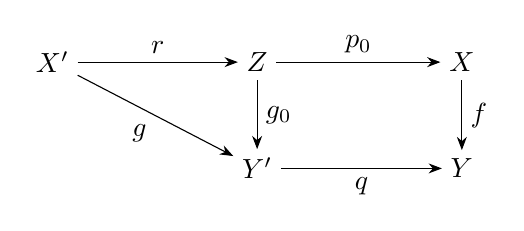
\begin{tikzpicture}[>=Stealth, every node/.style={inner sep=3pt}]
\node (Xp) at (0,1.35) {$X'$};
\node (Z) at (2.6,1.35) {$Z$};
\node (X) at (5.2,1.35) {$X$};
\node (Yp) at (2.6,0) {$Y'$};
\node (Y) at (5.2,0) {$Y$};
\draw[->] (Xp) -- node[above] {$r$} (Z);
\draw[->] (Z) -- node[above] {$p_0$} (X);
\draw[->] (Xp) -- node[below left] {$g$} (Yp);
\draw[->] (Z) -- node[right] {$g_0$} (Yp);
\draw[->] (X) -- node[right] {$f$} (Y);
\draw[->] (Yp) -- node[below] {$q$} (Y);
\end{tikzpicture}
\caption{The flattened main component $Z$ is equidimensional over
$Y'$.  A prime divisor on the resolution $X'$ whose image in $Y'$
has codimension at least two must therefore be exceptional for $r$.}
\label{desc:diagram}
\end{figure}

Put $\alpha=c_1(p^*M)$, choose a K\"ahler form $\omega$ on $X'$, and
choose a closed positive current $T$ representing $\alpha$.
The volume
\[
                  c=\int_{X'_y}\omega^d
\]
is positive and constant on the smooth-fibration locus.  Define the
closed positive $(1,1)$-current
\begin{equation}\label{desc:base-current}
                  S=c^{-1}g_*(T\wedge\omega^d)
\end{equation}
on $Y'$.  We claim that $T=g^*S$ over that locus.
Indeed $g_*(T\wedge\omega^{d-1})$ is a closed positive current of
degree zero, hence a nonnegative constant.  Its cohomology class is
the fiber intersection of $\alpha$ with $\omega^{d-1}$, which vanishes.
Thus this current is zero.  In local product coordinates this says
that the vertical block of the positive matrix of measures defining
$T$ vanishes.  Positivity also forces its mixed block to vanish.
Closedness then makes the horizontal coefficients independent of the
fiber coordinates.  Connectedness of the fibers makes these local
currents descend, and Equation~\eqref{desc:base-current} identifies
their common descent as $S$.

The current $S$ has local plurisubharmonic potentials, so its pullback
by the dominant map $g$ is defined on all of $X'$.
The closed order-zero current $T-g^*S$ is supported on the inverse
image of the complement of the smooth-fibration locus in $Y'$.
The support theorem for currents
\cite[Chapter~III, Corollaries~2.11 and~2.14]{DemaillyCADG} therefore gives
\begin{equation}\label{desc:vertical-difference}
              T-g^*S=[D],\qquad D=\sum_E x_E E,
\end{equation}
where $D$ is a signed real divisor supported on vertical primes.
We next show that its components dominating base divisors come in
whole pullbacks.

Fix a prime divisor $Q\subset Y'$ occurring among their images, and
let $E_1,\ldots,E_s$ be the primes of $X'$ dominating $Q$.
Let $a_i>0$ be their multiplicities in $g^*Q$, and let $x_i$ be their
coefficients in $D$.  For a K\"ahler form $\eta$ on $Y'$, set
\begin{equation}\label{desc:intersection-matrix}
       C_{ij}=\int_{X'}\{E_i\}\{E_j\}\,(g^*\eta)^{k-1}\omega^{d-1}.
\end{equation}
For $i\ne j$, these numbers are nonnegative.
The inverse image $g^{-1}(Q)$ is an effective Cartier divisor, hence
has pure codimension one.  After a generic choice of the point in
$Q$, its fiber components all have pure dimension $d$.  Distinct
primes $E_i,E_j$ have pure codimension-two intersection; if they
meet over a general point of $Q$, that intersection dominates $Q$
and has fibers of dimension $d-1$.  It therefore contributes
positively to $C_{ij}$.  These dimension statements follow by
generic flatness over $Q$, excluding the smaller base images.
The graph having an edge when $C_{ij}>0$ is consequently connected.  Indeed, over a general point
of $Q$ the irreducible components of the connected fiber have a
connected intersection graph.  Grouping those components according
to the global prime $E_i$ containing them gives the graph above as
a quotient, which is still connected.  Moreover $Ca=0$, where
$a=(a_i)$.
To see this, pair $E_i$ with $g^*Q$ and $(g^*\eta)^{k-1}\omega^{d-1}$.
Its image lies in $Q$, so the $k$ classes from the base give zero.
Components of $g^*Q$ whose images have codimension at least two give
zero separately in this pairing.

Let $\beta$ be the Bott--Chern class of $S$.  Equation~\eqref{desc:vertical-difference} gives
$\{D\}=\alpha-g^*\beta$.  Pairing this identity with each
$E_i(g^*\eta)^{k-1}\omega^{d-1}$ shows that
\[
                               Cx\geq0.
\]
Here the $\alpha$ term is nonnegative by nefness, and the base term
vanishes by dimension.  Components of $D$ above other base divisors,
or above sets of codimension at least two, also contribute zero.
Since $a$ has strictly positive entries and $a^{\mathsf t}Cx=0$,
we obtain $Cx=0$.  The kernel is precisely $\R a$: indeed
\[
 x^{\mathsf t}Cx
 =-\sum_{i<j} C_{ij}a_i a_j
       \left(\frac{x_i}{a_i}-\frac{x_j}{a_j}\right)^2,
\]
and the graph is connected.  Consequently $x_i=t_Qa_i$ for one
real number $t_Q$.

Subtract $g^*(\sum_Q t_QQ)$ from $D$, and denote the resulting divisor
by $D_0$.  Its image in $Y'$ has codimension at least two.
Equidimensionality of $g_0$ implies that every such prime on $X'$ is
$r$-exceptional.  Also
\[
 \{D_0\}=\alpha-g^*\beta',\qquad
 \beta'=\beta+\sum_Q t_Q\{Q\}.
\]
Both classes on the right come from classes with local potentials
on $Z$: $\alpha$ comes from the original source $X$, and $\beta'$
comes from $Y'$.  Thus $D_0$ has degree zero on every curve contracted
by $r$.  Relative negativity for a projective morphism of normal analytic
spaces \cite[Section~11, after Definition~11.1]{FujinoAnalyticBCHM}, applied to the exceptional divisors
$D_0$ and $-D_0$, gives $D_0=0$.  We have proved
\begin{equation}\label{desc:real-pullback}
                              \alpha=g^*\beta'.
\end{equation}

It remains to justify that the descended class is a rational line
class; the use of $\omega$ above does not supply rationality by
itself.  Pullback
\[
                    g^*:H^2(Y',\Q)\longrightarrow H^2(X',\Q)
\]
is injective.  Over $\R$ a left inverse is obtained by pushing
against $\omega^d$ and dividing by $c$, so injectivity follows there
and hence over $\Q$.  An injective rational linear map has a rational
preimage for every rational vector in its real image.  Since
$\alpha$ is rational, Equation~\eqref{desc:real-pullback} therefore
makes $\beta'$ rational.  It has type $(1,1)$, and the Lefschetz
$(1,1)$ theorem gives a rational line $N$ with $c_1(N)=\beta'$.

Finally suppose that $Y'$ is projective.  For any irreducible curve
$C\subset Y'$, resolve a component of $g^{-1}(C)$ that dominates
$C$, and factor its map through the normalization of $C$.
The pullback of $\alpha$ is nef.  Pairing it with a K\"ahler power
on that resolution gives a positive constant times $\deg(N|_C)$.
This degree is nonnegative.  The projective numerical criterion for
nefness now shows that $N$ is nef.
\end{proof}

The preceding proposition descends the Chern class.  For later use we
also need an actual rational-line identity.  The price is a single
flat twist on the original source.

\begin{corollary}[Choosing a descended representative]
\label{desc:representative}
In the notation and under the hypotheses of
Proposition~\ref{desc:nef}, there is a rational line $M^*$ on $X$
with $M^*\num M$ such that
\[
                          p^*M^*\qsim g^*N.
\]
\end{corollary}

\begin{proof}
The rational line $g^*N-p^*M$ has zero real Chern class.  After clearing
denominators and torsion, it belongs to $\Pic^0(X')$.
Lemma~\ref{pre:picard}(2) identifies $\Pic^0(X)$ with
$\Pic^0(X')$.  Thus
$g^*N-p^*M\qsim p^*F$ for some $F\in\Pic^0(X)\otimes\Q$.
Take $M^*=M+F$.
\end{proof}

The next lemma explains which fiberwise trivial flat twists already
come from the base.  Passing to rational lines allows us to remove
finite meridian holonomy and torsion Chern classes.

\begin{lemma}[Descent of a flat line]\label{desc:flat}
Let $f:X\to Y$ be a fibration of smooth connected compact K\"ahler
manifolds, and let $F\in\Pic^0(X)\otimes\Q$.
If $F$ is trivial as a rational line on a general smooth fiber, then
\[
                         F\qsim f^*G
\]
for some $G\in\Pic^0(Y)\otimes\Q$.
\end{lemma}

\begin{proof}
Take a positive multiple so that $F$ is a genuine unitary flat line
and its restriction to one smooth fiber $X_y$ is holomorphically
trivial.  On a compact connected K\"ahler manifold, a holomorphically
trivial unitary flat line has trivial holonomy.  Thus the character
of $F$ is trivial on $\pi_1(X_y)$.

Choose a dense Zariski open $Y^\circ$ over which $f$ is smooth, and
write $X^\circ=f^{-1}(Y^\circ)$.  The homotopy sequence of the smooth
proper fibration gives
\[
 \pi_1(X_y)\longrightarrow\pi_1(X^\circ)
       \longrightarrow\pi_1(Y^\circ)\longrightarrow1.
\]
The character of $F|_{X^\circ}$ therefore comes from a unitary
character $\chi$ of $\pi_1(Y^\circ)$.

Let $Q$ be a divisorial component of $Y\setminus Y^\circ$.
Choose a prime dominating $Q$ and a transverse disk at a general
point of that prime, away from the other components of the inverse
image of $Y\setminus Y^\circ$.  Its image winds $a_Q$ times around a small meridian
of $Q$, where $a_Q>0$ is the multiplicity of that prime in $f^*Q$.
The disk lies in $X$, so the character of $F$ is trivial on its
boundary.  Hence $\chi$ has finite order dividing $a_Q$ on the base
meridian.  There are finitely many such $Q$.  A common power of
$\chi$ kills all their meridians and therefore factors through
$\pi_1(Y)$; subsets of complex codimension at least two add no
obstruction.  The resulting unitary flat line on $Y$ has zero real
Chern class, and another power removes any torsion in its integral
Chern class.  It then belongs to $\Pic^0(Y)$.

The resulting characters agree after pullback on $X^\circ$.
Since $\pi_1(X^\circ)\to\pi_1(X)$ is surjective, they agree on $X$
as well.  Dividing by the powers taken in the argument proves the
asserted identity in $\Pic(X)\otimes\Q$.
\end{proof}

\section{An ordinary adjoint on the projective base}
\label{sec:adjoint}

The induction will produce a morphism to a projective variety for which an
ordinary adjoint is pulled back from the base.  To apply the projective
numerical-semiampleness theorem, we must realize the line downstairs as an
ordinary klt adjoint.  The following proposition provides this realization.
The total space need not be projective.

\begin{proposition}[An adjoint on the base]
\label{adj:base}
Let $(Y,D)$ be an effective klt pair with rational boundary on a normal
compact K\"ahler space.  Let $f:Y\to Z$ be a surjective morphism with connected
fibers to a normal projective variety, and suppose that
$\dim Y>\dim Z$.  If $H$ is a rational Cartier line bundle on $Z$ and
\begin{equation}
\label{adj:initial}
                         K_Y+D\qsim f^*H,
\end{equation}
then there is an effective rational divisor $D_Z$ such that $(Z,D_Z)$ is klt
and
\[
                         H\qsim K_Z+D_Z.
\]
\end{proposition}

Ambro proves the corresponding statement for projective total spaces
\cite[Theorem~0.2]{Ambro}.  We follow the same separation into a discriminant
and a Hodge-theoretic moduli line.  The two points requiring attention here
are the real, possibly irrational polarization of a K\"ahler family and the
construction of its cyclic cover without a meromorphic frame of $K_Y$.
The period results recalled next address the first point; we give the cover
and the required infinitesimal calculation explicitly.

\subsection{The period input and the discriminant}

For a pure variation of Hodge structures on a smooth open set, the
\emph{line period map} of a rank-one highest Hodge piece is the map to the
projective space of the flat vector space that records this line in a local
flat trivialization.  Its generic differential rank is independent of the
trivialization.  The full period map records the entire Hodge filtration.
For quasi-unipotent boundary monodromy, the \emph{parabolic extension} of the
line is the rational line bundle obtained by making the monodromy unipotent
on local finite covers, extending the highest Hodge piece, and descending
with its rational boundary weights.

We use the following precise consequence of the period results in
\cite[Lemmas~4.1 and~4.3 and Proposition~4.5]{LI}.

\begin{lemma}[Period quotient input]
\label{adj:period-input}
Let $S$ be a smooth projective variety and let $S^\circ\subset S$ have simple
normal crossing complement.  Let $\mathbb V$ be a real-polarizable pure
variation on $S^\circ$ with an integral lattice and quasi-unipotent local
monodromy.  Suppose that a complex direct summand of $\mathbb V_{\C}$, as a
variation of Hodge structures, has a rank-one highest Hodge piece, with parabolic extension $L$.  Then $L$ is nef,
and its numerical dimension is the generic rank of its line period map.

After modification $\tau:S'\to S$, there are a smooth projective variety
$Q$, a surjective morphism $p:S'\to Q$ with connected fibers, and a nef
rational line bundle $P$ on $Q$ such that
\begin{equation}
\label{adj:period-descent}
                         \tau^*L\qsim p^*P.
\end{equation}
Moreover, $\dim Q$ is at most the generic rank of the full period map of
$\mathbb V$.  If $Q$ is a point, $\tau^*L$ is rationally trivial.
\end{lemma}

Here the identity is in $\Pic(S')\otimes\Q$, including the boundary.
For clarity, the dimension assertion follows because the descended,
generically immersive period map on $Q$ belongs to an adjoint variation
obtained by tensor constructions from $\mathbb V$.
The rational adjoint reduction in \cite[Lemma~4.3]{LI} retains entire
rational simple factors, so its monodromy is discrete even when the
original real polarization is irrational.  It also kills only finite
scalar monodromy after taking a power.  Thus
\eqref{adj:period-descent} does not discard an arbitrary flat twist.
We shall need exactly this actual line identity.

Choose a projective resolution $b:S\to Z$, and normalize the main
component of $Y\times_Z S$.  Choose its log resolution functorially
with respect to local isomorphisms preserving the marked boundary;
over the open where $b$ is an isomorphism this is a functorial log
resolution of $(Y,D)$.  Denote the resulting smooth compact K\"ahler
space by $X$, with maps $\pi:X\to Y$ and $g:X\to S$.
Such a resolution is available in the complex analytic category;
see \cite[Theorem~1.1 and the preceding analytic remark]{BierstoneMilman2008}.
The functorial choice will matter when we lift local flows.
Additional resolutions used to compute thresholds and fiber integrals
are auxiliary and do not replace the family whose cohomology we use.
Define the crepant rational divisor $D_X$ by
\[
              K_X+D_X=\pi^*(K_Y+D).
\]
Its exceptional coefficients may be negative; all its coefficients are
strictly less than one.  For a prime divisor $Q_0$ on $S$, let
\[
 t_{Q_0}=\sup\{c\in\R:(X,D_X+c g^*Q_0)
             \text{ is log canonical over the general point of }Q_0\}.
\]
The definition is unchanged on a higher crepant resolution.  It gives a
positive rational number, computed by a log resolution as
\begin{equation}
\label{adj:threshold}
             t_{Q_0}=\min_i\frac{1-u_i}{a_i},
\end{equation}
where $g^*Q_0=\sum_i a_i E_i$ over its general point and $u_i$ is the
coefficient of $E_i$ in the crepant boundary there.  Define
\begin{equation}
\label{adj:discriminant}
 \Delta_S=\sum_{Q_0}(1-t_{Q_0})Q_0,
 \qquad L_S=b^*H-K_S-\Delta_S.
\end{equation}
Only finitely many terms of $\Delta_S$ are nonzero: off a suitable proper
analytic subset the resolved pair is relatively simple normal crossing,
the map is smooth, and the threshold of a base prime is one.  We may choose
$S$ with a simple normal crossing divisor containing this exceptional set
and the support of $\Delta_S$.

The coefficients of $\Delta_S$ are strictly less than one.  To prove
Proposition~\ref{adj:base}, we will show that $L_S$ has an effective rational
representative whose addition to $\Delta_S$ is sub-klt.  The relevant
positivity comes from the following root construction.

\subsection{The root cover and its highest Hodge line}

\begin{lemma}[The root eigenline]
\label{adj:root}
In the setting of Proposition~\ref{adj:base}, there is a dense Zariski open
$S^\circ\subset S$ and a smooth proper family $h:V^\circ\to S^\circ$ obtained
from a cyclic cover and resolution, such that $R^l h_*\R$, where
$l=\dim Y-\dim Z$, is real-polarizable and has an integral lattice.
One character summand of its complexification has a rank-one highest
Hodge piece.  On $S^\circ$, this line agrees, as a rational line bundle,
with $b^*H-K_S$.
\end{lemma}

\begin{proof}
Choose an integer $m>0$ clearing all divisors and rational line identities.
A meromorphic section of the line $m b^*H$ exists because $S$ is projective.
Its pullback, under the identity
\[
                m(K_X+D_X)\simeq g^*(m b^*H),
\]
and division by the canonical meromorphic section of $mD_X$ give a
meromorphic section $\sigma$ of $K_X^{\otimes m}$.
On the open where $\sigma$ has neither zeros nor poles, take its $m$th
roots in the fibers of $K_X$.  In local canonical frames this is the
equation $z^m=\sigma$; on overlaps the roots transform by the transition
functions of $K_X$.  The local covers therefore glue without a
meromorphic trivialization of $K_X$, and without choosing a root of $H$.

The Grauert--Remmert extension theorem for finite analytic covers
\cite[Exposé~XII, Proposition~5.3 and Theorem~5.4]{SGA1} extends it
normally across the divisor of $\sigma$, giving a finite cyclic cover
of $X$, possibly disconnected.  It is compact K\"ahler.
Take a resolution functorial for the cyclic action and for local
isomorphisms of the pair, as in \cite[Section~1.1 and Lemma~1.1]{Ambro}.
Thus both resolutions are functorial.  A local flow preserving the
original pair lifts through them once its lift to the root cover has
been chosen; we will construct that lift explicitly below.
The resulting compact manifold $V$ is K\"ahler.  After deleting from $S$ the zeros and
poles of the chosen base section and the degeneration locus, the map
$h:V^\circ\to S^\circ$ is smooth and proper.  We take $S^\circ$
inside the isomorphism locus of $b$.  Shrinking it further, the original
fibers of $Y\to Z$ are normal effective klt pairs and the chosen
resolutions restrict to resolutions of those pairs.

Average a global K\"ahler class on $V$ under the cyclic group.  Its
restriction is a flat real section of $R^2h_*\R$ and polarizes the
primitive pieces.  Their Lefschetz decomposition supplies a flat real
polarization of the full degree-$l$ cohomology.  We retain the full
cohomology local system, with lattice $R^lh_*\Z$ modulo torsion; an
irrational primitive summand is not required to carry its own lattice.
The finite group action preserves this variation and its polarization.

Locally over the base, the tautological root, divided by a local base
volume form, gives a relative meromorphic top form $\tau$ on the cover.
It belongs to a fixed character of the cyclic group.  The klt condition
makes its squared volume locally integrable, including after resolution,
so it extends holomorphically: a meromorphic top form with a divisorial
pole cannot be locally square integrable.
To see the orders directly, consider a boundary prime on the original
normal fiber with coefficient $u=p/e\in(0,1)$ in lowest terms.  At a
general point the cover has local coordinate $x=y^e$, and the pulled-back
root form has order
\begin{equation}
\label{adj:root-order}
                         e-1-eu=e-1-p\in\{0,\ldots,e-2\}.
\end{equation}
Away from the boundary its order at a nonexceptional prime is zero.
The corresponding calculation on a crepant resolution uses coefficients
less than one and proves integrability at exceptional divisors as well.

Suppose that $\tau'$ is another holomorphic top form of the same
character on a fiber.  The ratio $\tau'/\tau$ is an invariant meromorphic
function and descends to the original normal connected fiber.
A pole along a boundary prime downstairs would pull back with order at
least $e$, whereas \eqref{adj:root-order} permits only $e-2$ zeros of
$\tau$.  No such pole is possible.  Away from the boundary, $\tau$ has
no divisorial zeros downstairs.  Normality extends the ratio across
codimension two, and compactness makes it constant.  This also handles
a disconnected cover, since the full root group acts transitively on
its components over a connected fiber.  The highest Hodge piece of the
chosen character is therefore one-dimensional.

Finally, changing a local frame of $m b^*H$ changes the root by an
$m$th root of the corresponding base factor; changing the base volume
form contributes the inverse canonical transition.  Taking the $m$th tensor power removes
the finite root ambiguities.  These are precisely the transitions of
$m(b^*H-K_S)$, proving the asserted identity on $S^\circ$.
\end{proof}

\begin{lemma}[Extension across the discriminant]
\label{adj:extension}
The parabolic extension of the eigenline in Lemma~\ref{adj:root} is $L_S$
of \eqref{adj:discriminant}.  This identification persists on higher
smooth base models with simple normal crossing complement.
\end{lemma}

\begin{proof}
Fix a general point of a prime $Q_0=(t=0)$ on $S$.  We normalize the
root form by a nonvanishing local frame of $b^*H-K_S$.  More explicitly,
if the meromorphic section of $m b^*H$ chosen in Lemma~\ref{adj:root}
is $a$ times a nonvanishing local frame, divide its root by $a^{1/m}$
and by the local base volume form.  This is an ordinary frame after a
finite power substitution; the finite ambiguity is precisely part of
the parabolic convention.  Thus zeros or poles of the chosen meromorphic
base section do not enter the following exponent.
Tangential base coordinates may be treated as parameters.  On a log resolution,
\[
                         t=\prod_{i=1}^k x_i^{a_i}
\]
up to a nowhere-zero factor, and the squared absolute root form has
vertical density factors $|x_i|^{-2u_i}$.  Horizontal boundary factors
are integrable because their coefficients are less than one.
The squared Hodge norm of the relative form is its fiber integral.
Writing $s_i=-\log|x_i|$, the integral is computed on slices
\[
                 \sum_i a_i s_i=-\log|t|
\]
with exponential weight $\exp(-2\sum_i(1-u_i)s_i)$.
Conversion to the ordinary base area element contributes $|t|^{-2}$.
The minimum in \eqref{adj:threshold} thus gives constants $C,N>0$ such
that, on a sufficiently small punctured disk,
\begin{equation}
\label{adj:norm-power}
 C^{-1}|t|^{2(t_{Q_0}-1)}(-\log|t|)^{-N}
 \leq \|\tau\|^2
 \leq C|t|^{2(t_{Q_0}-1)}(-\log|t|)^N.
\end{equation}
Indeed, the slice has at most polynomial volume in $-\log|t|$, which
proves the upper estimate after factoring out the least exponential
decay.  For the lower estimate take a chart along a component attaining
the minimum, away from all other vertical components, and integrate
over a fixed compact set in the remaining directions.  Compactness
allows finitely many charts; the integrable horizontal factors do not
alter the power of $|t|$.

After a local power substitution making monodromy unipotent, extending
Hodge frames and their duals have norms bounded by powers of
$-\log|t|$.  These are the nilpotent-orbit estimates of
Schmid and Cattani--Kaplan--Schmid \cite{Schmid,CKS}, in the form used in
\cite[Section~4.1]{LI}.  Consequently the comparison between a
frame of $b^*H-K_S$ and an extending Hodge frame has rational order
$t_{Q_0}-1$.  Multiplication by $t^{1-t_{Q_0}}$, on a cover where this
power is integral, removes exactly that order.  Both the corrected
comparison and its inverse have at most logarithmic growth.  A
holomorphic function on a punctured disk with such growth has no pole;
applying this to the inverse excludes a zero.  The same argument with
tangential parameters extends the identification across each divisor,
and normal extension treats codimension two.  Thus the extending line is
\[
              b^*H-K_S+\sum_{Q_0}(t_{Q_0}-1)Q_0=L_S.
\]
For the last assertion, first make the boundary monodromies
unipotent.  In canonical extending frames a local monomial pullback
$t_i=\text{unit}\cdot\prod_j s_j^{a_{ij}}$ replaces the commuting
nilpotent residues $N_i$ by $\sum_i a_{ij}N_i$, which are again
nilpotent.  Both the canonical flat extension and its extending Hodge
filtration therefore pull back without an additional divisor.
Descending with rational weights incorporates the finite-monodromy
parts and gives the same conclusion for the parabolic line, including
exceptional base divisors; see \cite[Section~4]{LI}.
\end{proof}

We have now identified the moduli line with an extreme Hodge line, so
Lemma~\ref{adj:period-input} makes it nef and gives an actual line
descent.  To obtain a big line on the quotient, we must compare the
variation seen by this one line with that seen by the whole family.
Effectivity of the original boundary is decisive in this comparison.

\subsection{The line detects the full period rank}

\begin{lemma}[Equality of period ranks]
\label{adj:rank}
For the family of Lemma~\ref{adj:root}, the line period map of its root
eigenline and the full period map of $R^lh_*\R$ have the same generic
differential rank.
\end{lemma}

\begin{proof}
Work in an open patch on which the ranks are constant, and let $\xi$
be a holomorphic base vector field in the kernel of the line period
map.  Choose a local frame $\tau$ of the eigenline, viewed as a
relative top form on $V^\circ$.  The infinitesimal period formula says
that contraction with $\tau$ sends the Kodaira--Spencer class of $\xi$
to zero in the fiber cohomology $H^1(\Omega^{l-1})$.

Here is the corresponding lifting construction.  Pull back the tangent
sequence to the line generated by $\xi$ and push it out along
\[
 T_{V^\circ/S^\circ}\longrightarrow
 T_{V^\circ/S^\circ}\otimes K_{V^\circ/S^\circ}
       \simeq\Omega^{l-1}_{V^\circ/S^\circ},
 \qquad v\longmapsto\iota_v\tau.
\]
Write $U$ for a sufficiently small Stein base patch and put
$\mathcal F=\Omega^{l-1}_{V_U/U}$.  The pushed-out extension is
\[
             0\longrightarrow\mathcal F
               \longrightarrow\mathcal E
               \longrightarrow\cO_{V_U}\longrightarrow0,
\]
with class in $H^1(V_U,\mathcal F)$.  Shrink within the generic locus
so that $R^1h_*\mathcal F$ is locally free and coherent base change
holds.  The contraction formula makes the image of this class in
$H^0(U,R^1h_*\mathcal F)$ zero.  The Leray exact sequence and the
vanishing $H^1(U,h_*\mathcal F)=0$ show that
$H^1(V_U,\mathcal F)\to H^0(U,R^1h_*\mathcal F)$ is injective.
The extension class is therefore zero, and a holomorphic splitting
exists on the entire $V_U$.
Where $\tau$ is nonzero, divide the vertical part of the splitting by
$\tau$.  This gives a meromorphic vector field $\widetilde\xi$ on the
resolved cover projecting to $\xi$, with poles bounded by the zero
divisor of $\tau$.  Average it under the root group.  Its projection
remains $\xi$, and the averaged field is invariant.

We check this field at codimension-one points of the original normal
total space.  At a boundary prime use the ramification coordinate
$x=y^e$ from \eqref{adj:root-order}.  A tangential coefficient of an
invariant vector field has Laurent exponents congruent to zero modulo
$e$.  Its permitted pole order is at most $e-2$, so every exponent is
nonnegative.  The coefficient of $\partial/\partial y$ has exponents
congruent to one modulo $e$.  Its first possible negative exponent is
$1-e$, which is again excluded.  The normal coefficient is therefore
divisible by $y$.  Thus the descended vector field is holomorphic and
tangent to the boundary.  At a prime outside the boundary the root
form has no zero, and the conclusion is immediate.

The resolution is an isomorphism at the codimension-one points just
used.  Remaining exceptional divisors map into codimension at least
two in the original normal space.  Holomorphic derivations extend
across that subset, so the descended field is holomorphic everywhere
on the family over our base patch and still projects to $\xi$.
Its local flow preserves the boundary components, their coefficients,
and the singular locus.  By the functorial choice made above, the flow
first lifts to $X$ and preserves its crepant boundary $D_X$.

This flow then lifts holomorphically to the root cover.  Indeed, on the good
base patch the defining pluriform has divisor exactly the negative
multiple of the boundary.  Pullback by a pair-preserving flow gives a
pluriform with the same divisor.  Their ratio is a holomorphic unit on
the normal space; its $m$th root can be chosen starting at one in the
flow parameter.  The root normalized at flow time zero is unique as a germ.  Thus the
local cover lifts agree on overlaps of the unbranched open and glue
by normality.  Functorial
resolution then lifts the flow to $V^\circ$.
Consequently the Kodaira--Spencer class of the resolved family vanishes
on $\xi$, and so does its full period differential.
The reverse kernel inclusion holds because the line is part of the
full Hodge filtration.  The two kernels, and therefore the generic
ranks, are equal.
\end{proof}

The argument is the analytic counterpart of Ambro's infinitesimal
comparison \cite[Proposition~2.1]{Ambro}.  Notice exactly where it uses
$D\geq0$: the strict pole bound in \eqref{adj:root-order} is imposed at
primes of the original pair.  Negative crepant exceptional coefficients
are allowed because their images have codimension at least two.

\subsection{Replacing the moduli line by a klt boundary}

\begin{proof}[Proof of Proposition~\ref{adj:base}]
Apply Lemma~\ref{adj:period-input} to the variation of
Lemma~\ref{adj:root}.  Its monodromy is quasi-unipotent by the monodromy
theorem for this proper K\"ahler family \cite{Schmid}.  Lemma~\ref{adj:extension}
identifies its parabolic line with $L_S$.  Passing to the indicated
higher smooth projective model, and keeping the notation $S$, we have
\[
                         L_S\qsim p^*P
\]
for a nef rational line $P$ on a smooth projective quotient $Q$.
Let $r$ be the generic rank of the line period map.  Numerical dimension
of a nef line is unchanged by a surjective pullback, so
\[
 r=\nu(L_S)=\nu(P)\leq\dim Q
       \leq\operatorname{rank}(d\Phi)=r,
\]
where $\Phi$ is the full period map and the last equality is
Lemma~\ref{adj:rank}.  Thus $P$ is big if $\dim Q>0$.  If $Q$ is a point,
$L_S$ is rationally trivial.

Suppose first that $\dim Q>0$.  By Kodaira's lemma write
$P\qsim A+E$, with $A$ ample rational and $E\geq0$ rational.  For every
small positive rational $\varepsilon$,
\begin{equation}
\label{adj:small-fixed-part}
 P\qsim A_\varepsilon+\varepsilon E,
 \qquad A_\varepsilon=(1-\varepsilon)P+\varepsilon A
                 \quad\text{ample}.
\end{equation}
The pair $(S,\Delta_S)$ is sub-klt.  On a fixed log resolution of
$\Delta_S+p^*E$, choose $\varepsilon$ sufficiently small that
$(S,\Delta_S+\varepsilon p^*E)$ remains sub-klt.  Choose a sufficiently
large divisible integer $N$ and a general member
$G\in|N A_\varepsilon|$.  The system $|Np^*A_\varepsilon|$ is
basepoint-free; on that resolution its general member meets the fixed
boundary transversely.  Taking $N$ large makes its coefficient $1/N$
less than one.  Bertini therefore gives an effective rational divisor
\[
                    E_S=\varepsilon p^*E+\frac1N p^*G
                    \qsim L_S
\]
with $(S,\Delta_S+E_S)$ sub-klt.  In the point case take $E_S=0$.
In either case,
\begin{equation}
\label{adj:upstairs-presentation}
                 K_S+\Delta_S+E_S\qsim b^*H.
\end{equation}

Set $D_Z=b_*(\Delta_S+E_S)$.  This divisor is effective.  Indeed, for
each prime of the original normal base, some component of its pullback
on $Y$ dominates it.  That component has multiplicity $a\geq1$ and
boundary coefficient $u\geq0$, so its threshold is at most
$(1-u)/a\leq1$.  Thus the coefficient of the discriminant at every
nonexceptional base prime is nonnegative, and $E_S$ is effective.

Choose compatible canonical divisors and a rational Cartier divisor
representing $H$.  The line identity
\eqref{adj:upstairs-presentation} gives an integer $m>0$ and a rational
function $\varphi$ in the common function field of $S$ and $Z$ such that
\[
 K_S+\Delta_S+E_S-b^*H=\frac1m\operatorname{div}_S(\varphi).
\]
Pushing down gives
\[
 K_Z+D_Z-H=\frac1m\operatorname{div}_Z(\varphi).
\]
In particular, $K_Z+D_Z$ is rational Cartier and rationally linearly
equivalent to $H$.  Pulling the latter divisor equality back and
comparing with the former proves the crepant identity
\[
                 K_S+\Delta_S+E_S=b^*(K_Z+D_Z).
\]
Since the pair upstairs is sub-klt, the effective pair $(Z,D_Z)$ is klt.
This proves the proposition.
\end{proof}

\section{Nef classes in algebraic dimension zero}\label{sec:zero}

A semiample line bundle on a space of algebraic dimension zero is
rationally trivial.  The induction therefore requires a stronger
conclusion in this case: the additional nef class must itself vanish.
The ordinary adjoint decomposition reduces this assertion to a question
about nef line bundles on simple manifolds.  We first carry out that
geometric reduction.  The remaining argument adapts the meromorphic
nonvanishing construction of \cite[Section~6]{K} to a line bundle that
need not be canonical.

\begin{proposition}\label{zero:vanishing}
Let \(n\ge1\).  Assume that the algebraic-dimension-zero assertion of
Theorem~\ref{thm:decomposition} holds in every dimension less than \(n\).
Let \(T\) be a smooth connected compact Kähler \(n\)-fold with
\(a(T)=0\), and let \(B\) be an effective rational simple normal crossing
boundary with coefficients less than one.  If \(K_T+B\) is
pseudo-effective, then every nef rational holomorphic line bundle \(M\)
on \(T\) satisfies \(c_1(M)=0\).
\end{proposition}

For intersections in this Section, a line bundle and its first Chern
class are distinguished when necessary by braces: \(\{H\}=c_1(H)\).
An inequality between real \((1,1)\)-classes is in pseudo-effective
order.  A compact manifold is \emph{simple} if no positive-dimensional
proper compact analytic subvariety passes through a very general point.
Here, as usual, ``very general'' permits deletion of a countable union
of proper analytic subsets.

\subsection{Reduction to a simple symplectic manifold}

The following elementary intersection test lets us use finite covers
without requiring the nef line bundle to descend through them.

\begin{lemma}\label{zero:mass-test}
Let \(V\) be a smooth compact Kähler \(n\)-fold, where \(n\ge1\),
and let \(\gamma\) be a nef
class, and let \(C\) be a nef and big class.  If
\(\gamma\cdot C^{n-1}=0\), then \(\gamma=0\).
In particular, if \(V\) admits a generically finite surjective morphism
to a complex torus of algebraic dimension zero, every nef rational line
class on \(V\) is zero.
\end{lemma}

\begin{proof}
Choose a Kähler class \(\omega\) and \(\varepsilon>0\) such that
\(C-\varepsilon\omega\) is pseudo-effective.  When \(n\ge2\), the
identity
\[
 C^{n-1}-(\varepsilon\omega)^{n-1}
 =(C-\varepsilon\omega)
   \sum_{j=0}^{n-2}C^{n-2-j}(\varepsilon\omega)^j
\]
and nonnegativity of intersections of a pseudo-effective class with
nef classes give
\[
 0=\gamma\cdot C^{n-1}
 \ge \varepsilon^{n-1}\gamma\cdot\omega^{n-1}\ge0.
\]
The same conclusion is immediate when \(n=1\).  A positive current in
\(\gamma\) thus has zero mass, so it vanishes.

For the last assertion, write \(f:V\to A\) for the morphism.  The
pushforward of the nef rational line class is a rational
pseudo-effective \((1,1)\)-class on \(A\).  Averaging a positive current
under translations represents it by a constant semipositive form.  The
kernel of a rational such form is the tangent space of a subtorus; the
induced positive integral form, after clearing denominators, polarizes
the quotient.  Since \(a(A)=0\), this quotient is a point, and hence
\(f_*\gamma=0\).  For a Kähler class \(\eta\) on \(A\), the class
\(C=f^*\eta\) is nef and big and
\[
 \gamma\cdot C^{n-1}=(f_*\gamma)\cdot\eta^{n-1}=0.
\]
Apply the first assertion.
\end{proof}

\begin{lemma}\label{zero:geometric-reduction}
Under the induction hypothesis of Proposition~\ref{zero:vanishing},
it suffices to prove the following assertion: every nef rational line
class on a smooth simple compact Kähler manifold of algebraic dimension
zero carrying a generically nondegenerate holomorphic two-form is zero.
\end{lemma}

\begin{proof}
Apply the ordinary good divisorial decomposition to \(K_T+B\).  On a
smooth modification its semiample part is rationally trivial, because
\(a(T)=0\).  After the klt modification convention of
Section~\ref{sec:preliminaries}, the resulting ordinary adjoint still
equals its rational negative divisor as an actual rational line bundle.
The contraction of a known negative part
\cite[Theorem~2.13 and Proposition~3.8]{K}, with nef part zero, produces
an ordinary compact Kähler klt pair \((T_0,B_0)\) such that
\(K_{T_0}+B_0\qsim0\).

The decomposition theorem of Matsumura--Wang--Wu--Zhang
\cite[Corollary~1.4]{BBYv2} applies to this pair: its nef b-part is zero.
A finite quasi-étale cover of \(T_0\) is a product of a rationally
connected factor, strict Calabi--Yau factors, irreducible holomorphic
symplectic factors, and a torus.  Algebraic dimension is unchanged by
proper generically finite maps and by modifications.  No
positive-dimensional rationally connected factor can occur, since a
Kähler resolution of such a factor is projective by algebraic
connectedness \cite{Campana1981}.  A strict Calabi--Yau factor of
dimension at least three has no holomorphic two-forms.  Extension of
forms for klt spaces \cite{KebekusSchnell2021} gives the same vanishing on a resolution, which is
projective by Kodaira's criterion.  Such factors are also excluded.
Dimension-two factors of Calabi--Yau type are counted among the
symplectic factors.  A resolution of an irreducible symplectic factor
has \(h^{2,0}=1\), generated by a generically nondegenerate form.

Resolve the cover and the maps to \(T\) and to smooth models of all its
factors.  We obtain a smooth compact Kähler manifold \(V\), with the
pulled-back nef line class \(\gamma\), mapping generically finitely to
\(T\) and to a product \(X_1\times\cdots\times X_r\).  If \(r\ge2\),
let \(C\) be the pullback of a sum of Kähler classes from the factors.
For the projection omitting \(X_i\), every component of a smooth general
fiber maps generically finitely to \(X_i\).  This fiber has algebraic
dimension zero and a nonzero top form, obtained by pulling back either
a torus volume form or a power of a symplectic form.  Its canonical class
is therefore pseudo-effective.  Its dimension is less than \(n\), so
the induction hypothesis, with zero boundary, makes the restriction of
\(\gamma\) zero.

Expand \(C^{n-1}\).  A nonzero term has top powers from all factors
except one, where precisely one power is missing.  Integration over the
fibers just considered shows that its pairing with \(\gamma\) is zero.
Thus \(\gamma\cdot C^{n-1}=0\), and Lemma~\ref{zero:mass-test} gives
\(\gamma=0\).  Vanishing descends to \(T\) by push--pull for a
generically finite map.  A single torus factor is covered by the last
assertion of that lemma.

It remains to consider one symplectic factor.  On a smooth model \(X\)
we have \(a(X)=0\) and \(H^0(X,\Omega_X^2)=\C\sigma\), with
\(\sigma\) generically nondegenerate.  There is no dominant meromorphic
fibration from \(X\) to an intermediate-dimensional compact base.
Indeed, on smooth Kähler models such a base has algebraic dimension
zero, hence is nonprojective and has a nonzero holomorphic two-form by
Kodaira's criterion.  Its pullback would be a nonzero degenerate
holomorphic two-form on \(X\), which is impossible.

The minimal-fibration theorem of Campana, in the form
\cite[Theorem~2.3(3) and Corollary~2.5(2)]{COP}, now says that \(X\)
is isotypically semi-simple.  This means that \(X\) and a power
\(S^r\) of a simple manifold have a common generically finite cover;
we may take smooth Kähler models.  If \(r\ge2\), repeat the preceding
product intersection argument.  The smaller-dimensional fibers are
simple: simplicity is preserved by generically finite maps between
spaces of algebraic dimension zero.  Indeed, a covering family of
proper subvarieties upstairs or downstairs gives such a family on the
other space by images or inverse images at points where the map is
finite; the countability of compact cycle components gives the very
general formulation.  They are not uniruled, and hence
their canonical bundles are pseudo-effective by \cite[Theorem~1.1]{Ou}.
The induction hypothesis again applies.  If \(r=1\), the common smooth
cover is simple and carries the pullback of \(\sigma\), a generically
nondegenerate holomorphic two-form.  This is precisely the assertion
stated in the lemma.
\end{proof}

\subsection{Finite correspondences and cotangent slopes}

We next isolate the two geometric properties needed for the
nonvanishing argument.  The first controls subvarieties of a product;
the second controls line subsheaves of cotangent tensors.

\begin{lemma}\label{zero:no-correspondences}
Let \(X\) be a smooth simple compact Kähler manifold of algebraic
dimension zero, carrying a generically nondegenerate holomorphic
two-form.  Suppose that every smooth connected compact Kähler manifold
mapping generically finitely onto \(X\) has irregularity zero.
Through a very general point of \(X^2\), the only positive-dimensional
proper irreducible compact analytic subvarieties are the two factor
slices.
\end{lemma}

\begin{proof}
Fix a generically nondegenerate holomorphic two-form \(\sigma\) on
\(X\).  A moving correspondence would produce a holomorphic one-form
on a fixed finite cover of \(X\).  To see this, we identify its first projection
with a fixed finite cover over a parameter ball, and then contract the
pulled-back two-form in a direction varying the second projection.

For a subvariety through a pair whose coordinates are very general,
simplicity makes each projection image either a point or all of \(X\).
If both projections dominate, their fibers through general points are
either zero-dimensional or the full other factor.  A proper such
subvariety must therefore be a generically finite correspondence.

Suppose these correspondences sweep \(X^2\).  The compact cycle spaces
of a compact Kähler manifold have countably many compact irreducible
components \cite{LiebermanCycles}.  One component must have incidence
image equal to \(X^2\).  Resolve that component and the relevant
incidence component, obtaining a compact Kähler parameter space \(S\),
a smooth incidence space \(Y\), and maps
\[
 h:Y\longrightarrow S,\qquad F_1,F_2:Y\longrightarrow X.
\]
For a general parameter, the fiber is smooth and irreducible, and each
\(F_i\) restricts to a generically finite map.  The map
\((F_1,h):Y\to X\times S\) is generically finite.  Its normal finite
Stein factor is a finite cover of the smooth product.

By purity, the branch locus of this cover is divisorial.  Every branch
component dominating \(S\) has a proper image in \(X\): otherwise its
divisorial fibers over \(S\) would sweep \(X\), contradicting
simplicity.  Compactness of \(S\) makes these images closed analytic
subsets.  Remove the images in \(S\) of the remaining branch components
and take a small ball \(B\) about a general parameter.  There is a fixed
proper analytic subset \(A\subset X\) such that the cover is étale
over \((X\setminus A)\times B\).  Since \(B\) is simply connected,
this étale cover is pulled back from a fixed cover of \(X\setminus A\).
Normalize \(X\) in that cover.  Uniqueness of normal finite extension
then identifies the cover over \(X\times B\) with the product of this
fixed normal cover and \(B\); see
\cite[Exposé~XII, Proposition~5.3 and Theorem~5.4]{SGA1}.

Let \(\widetilde X\) be a smooth Kähler resolution of the fixed cover.
The second projection gives a meromorphic map
\(G:\widetilde X\times B\dashrightarrow X\).  The pullback \(G^*\sigma\)
is a holomorphic two-form: resolve the meromorphic map and descend
holomorphic forms across a modification of a smooth space.  Dominance
of \((F_1,F_2)\) implies that, at suitable general points, the
derivatives of \(G\) in the parameter directions span \(T_X\), while
the derivative along \(\widetilde X\) is an isomorphism.  Choose a
constant tangent vector on \(B\) for which this parameter derivative
is nonzero at such a point.  Contracting \(G^*\sigma\) with that vector
and restricting to \(\widetilde X\times\{t\}\) yields a nonzero global
holomorphic one-form on \(\widetilde X\).  This contradicts the
hypothesis on irregularity.

Each component parametrizing generically finite correspondences thus
has proper incidence image.  Their countable union misses a very
general pair, proving the assertion.
\end{proof}

\begin{lemma}\label{zero:cotangent-slope}
Let \(X\) be a smooth simple compact Kähler manifold of dimension
\(n\ge2\), algebraic dimension zero and irregularity zero, and suppose \(K_X\) is
pseudo-effective.  Let \(\mathscr L\) be a holomorphic line bundle such
that \(L=c_1(\mathscr L)\ge c_1(K_X)\) in pseudo-effective order.
For every nonzero map \(\mathscr H\to\Omega_X^{\otimes k}\), where
\(\mathscr H\) is a line bundle and \(k\ge0\),
\begin{equation}\label{zero:slope-X}
 c_1(\mathscr H)\le kL.
\end{equation}
For every very general \(x\in X\), write
\(a:Y=\operatorname{Bl}_xX\to X\).  Every nonzero line map
\(\mathscr H_Y\to(a^*\Omega_X)^{\otimes k}\) satisfies
\begin{equation}\label{zero:slope-blowup}
 c_1(\mathscr H_Y)\le ka^*L.
\end{equation}
The exceptional set of points can be chosen simultaneously for all
\(\mathscr H_Y\) and \(k\).
\end{lemma}

\begin{proof}
We give the slope argument from \cite[Lemma~6.2]{K}, indicating why it
does not require any hypothesis about canonical sections.  Let
\(\gamma\) belong to the full dual of the pseudo-effective cone.
Ou's convention calls precisely these classes movable, and
Harder--Narasimhan filtrations exist for them
\cite[Definition~4.2 and Lemma~4.3]{Ou}.  If the minimum
\(\gamma\)-slope of \(\Omega_X\) were negative, the first
Harder--Narasimhan subsheaf \(\mathscr T\subset T_X\) would have
positive slope and be semistable.  Tensor slope inequalities make its
bracket into \(T_X/\mathscr T\) zero, so it is a foliation.  Its dual
has negative maximum slope and is non-pseudo-effective.  By
\cite[Theorem~1.4, Lemmas~4.3--4.4 and Proposition~4.5]{Ou}, its leaves have
compact closures given by a meromorphic fibration.  The rank of
\(\mathscr T\) is strictly less than \(\dim X\), since
\(c_1(T_X)\cdot\gamma\le0\).  A general leaf closure contradicts
simplicity.

All Harder--Narasimhan quotient slopes of \(\Omega_X\) are consequently
nonnegative, and its maximum slope is at most
\(c_1(K_X)\cdot\gamma\).  Tensor slopes give
\[
 c_1(\mathscr H)\cdot\gamma
 \le k c_1(K_X)\cdot\gamma\le kL\cdot\gamma.
\]
Separation by the dual cone proves \eqref{zero:slope-X}.

Irregularity zero embeds \(\Pic(X)\) in the countable group
\(H^2(X,\Z)\).  For any vector bundle on \(X\), linearly independent
global sections are generically pointwise independent: the coefficients
expressing one section in a maximal pointwise independent subfamily
are meromorphic functions, hence constants because \(a(X)=0\).
Evaluation is therefore injective outside a proper analytic subset.
Apply this simultaneously to
\(\mathscr H^{-1}\otimes\Omega_X^{\otimes k}\) for all lines
\(\mathscr H\) and all \(k\).

For a point outside the resulting countable exceptional union, write
\(\mathscr H_Y=a^*\mathscr H\otimes\cO_Y(mF)\), where \(F\) is the
exceptional divisor.  A nonzero map as in the statement extends away
from \(F\) to a section on \(X\) by Hartogs.  If \(m>0\), that section
vanishes at \(x\), because \(a_*\cO_Y(-mF)=\mathcal I_x^m\),
contrary to injectivity of evaluation.  Thus \(m\le0\), and
\eqref{zero:slope-X} proves \eqref{zero:slope-blowup}.
\end{proof}

\subsection{Meromorphic nonvanishing from cotangent slope bounds}

The next proposition extracts the line-bundle content of the
construction in \cite[Section~6]{K}.  Its hypotheses deliberately separate
cotangent slopes from the identity of the chosen line bundle.  This is
what permits the application to the sum of the canonical bundle and a
nef line bundle.

\begin{proposition}\label{zero:line-nonvanishing}
Let \(X\) be a smooth simple compact Kähler manifold of dimension
\(n\ge2\), with \(a(X)=0\) and irregularity zero.  Assume that the only
positive-dimensional proper compact irreducible analytic subvarieties
through a very general point of \(X^2\) are its factor slices.
Let \(\mathscr L\) be a holomorphic line bundle with pseudo-effective
class \(L\).  Assume the following line-subsheaf bounds:
\begin{enumerate}
\item For every line bundle \(\mathscr H\), every integer \(k\ge0\),
and every nonzero map \(\mathscr H\to\Omega_X^{\otimes k}\), one has
\(c_1(\mathscr H)\le kL\).
\item Outside a countable union of proper analytic subsets of \(X\),
every point \(x\) has this property: if
\(a:Y=\operatorname{Bl}_xX\to X\), then for every line bundle
\(\mathscr H_Y\), every \(k\ge0\), and every nonzero map
\(\mathscr H_Y\to(a^*\Omega_X)^{\otimes k}\), one has
\(c_1(\mathscr H_Y)\le ka^*L\).
\end{enumerate}
Then some positive power of \(\mathscr L\) has a nonzero meromorphic
section.
\end{proposition}

We prove the proposition by comparing point poles with vanishing along
a diagonal.  Assume, throughout the proof, that no positive power of
\(\mathscr L\) has a nonzero meromorphic section.  A normalized big class
on \(X\) has bounded pole order at a very general point.  On the rank-two projective bundle over \(X^2\) formed from the two
pullbacks of \(\mathscr L\), a class of growing volume produces a
large family of symmetric cotangent tensors.
The diagonal in \(X^2\) forces a large common vanishing order in
their determinant.  The slope inequalities then turn that vanishing into an
impossible point pole on \(X\).

The proof below follows the volume and two-diagonal construction of
\cite[results~6.3--6.10]{K}.  We retain its analytic estimates and give
their proofs along with the determinant calculations, so that the
chosen line bundle enters only through the hypotheses stated above.

\subsubsection{Point pole thresholds}

We will use several standard facts about volumes of real \((1,1)\)-classes.
Our normalization is \(\operatorname{vol}(\alpha)=\int\alpha^e\) for a nef class on an
\(e\)-fold.  Volume is continuous, homogeneous, monotone in
pseudo-effective order, invariant under modification, and its \(e\)-th
root is concave on the big cone.  Analytic Fujita approximation computes
it by Kähler parts on smooth projective modifications.  Here a
\emph{smooth projective modification} means a projective modification
whose source is smooth; the sources used here are compact Kähler
manifolds obtained by resolving coherent analytic ideals.  For a smooth
irreducible divisor \(D\) and a big class \(\alpha\), write
\(\operatorname{vol}_{\,|D}(\alpha)\) for the numerical restricted volume.
It is zero when \(D\) is contained in the non-Kähler locus
\cite[Theorem~1.1]{Vu2023}; otherwise it is
the supremum of the masses on \(D\) of restrictions of Kähler currents
with analytic singularities that are not generically singular on \(D\)
\cite[Lemma~2.7]{CollinsTosatti2018}.  The divisorial derivative and its
continuity on the big cone are
\begin{equation}\label{zero:volume-derivative}
 \frac{\mathrm{d}}{\mathrm{d} u}\operatorname{vol}(\alpha-u\{D\})
   =-e\,\operatorname{vol}_{\,|D}(\alpha-u\{D\});
\end{equation}
see \cite[Theorem~1.1]{Vu2023}.  We apply this formula only on smooth
manifolds while the varying class is big.

Here is a useful precise form of the approximation in the restricted
volume formula.  Resolve the log-ideal singularities of a current
restricted to \(D\).  Its pullback is an effective real divisor plus a
positive residual current with locally bounded potentials.  The latter
dominates a positive multiple of the pulled-back Kähler form.  A current
with locally bounded potentials has zero Lelong numbers, so Demailly
regularization makes its class, after subtracting that multiple, nef
\cite[Theorem~1.1]{DemaillyRegularization1992}.
On a projective modification there is an effective exceptional divisor
whose negative is relatively ample.  Subtracting a sufficiently small
multiple of this divisor from the residual class therefore makes that
class Kähler; add the same multiple to the divisor part.  Round all
divisor coefficients slightly upwards to rational numbers.  Openness of
the Kähler cone preserves the Kähler property.  These changes can be
arbitrarily small in top intersections, which compute the original mass
by the bounded-potential product formula.  Thus we may approximate a
restricted mass by
\begin{equation}\label{zero:rational-fujita}
 h^*(\alpha|_D)=\beta+\{D'\},\qquad
 \beta\ \text{Kähler},\quad D'\ge0\ \text{a rational divisor}.
\end{equation}
Moreover, \(D'\) has at least the log-ideal orders of the original
restriction on every further resolution.  We will use this last
property to turn poles into vanishing conditions.  Only \(D'\) is made
rational; the class \(\beta\) and the horizontal part of \(\alpha\) remain
real.

\begin{lemma}[A point pole bound]\label{zero:pole-threshold}
Let \(W\) be a smooth compact Kähler manifold of dimension \(e\ge2\),
\(\alpha\) a big real \((1,1)\)-class, and \(z\in W\).  Suppose a smooth
projective modification \(\mu:W'\to W\), which is an isomorphism near
\(z\), admits a decomposition
\[
 \mu^*\alpha=K+\{D\},\qquad K\ \text{Kähler},\quad D\ge0,
\]
where \(D\) misses the point \(z'\) over \(z\).  If the ordinary analytic
Seshadri constant \(\epsilon(K,z')\) is at least \(\eta>0\), then, on the
blowup \(b:\widehat W=\operatorname{Bl}_zW\to W\) with exceptional divisor \(G\),
\begin{equation}\label{zero:pole-formula}
 \sup\{u\ge0:b^*\alpha-u\{G\}\ge0\}
 \le \frac{\eta}{2}
     +2^{e-1}\operatorname{vol}(\alpha)\eta^{-(e-1)} .
\end{equation}
\end{lemma}

\begin{proof}
Set \(u_0=\eta/2\).  Blowing up \(z'\), the class
\(K-u_0\{G'\}\) is Kähler.  The Fujita decomposition is unchanged near
\(G'\), so it supplies a Kähler current for
\(\alpha_{u_0}=b^*\alpha-u_0\{G\}\) that is smooth near \(G\).
Its restriction there has class \(u_0c_1(\cO_{\mathbb{P}^{e-1}}(1))\).
The restricted volume is consequently \(u_0^{e-1}\): the current gives
this lower bound, and the volume of the restricted class gives the
opposite bound.

Let \(\tau\) denote the left side of Equation~\eqref{zero:pole-formula}.  The classes
\(\alpha_u=b^*\alpha-u\{G\}\) are big for \(0\le u<\tau\), since
\(\alpha_0\) is big and the pseudo-effective cone is convex.  The
concave function \(f(u)=\operatorname{vol}(\alpha_u)^{1/e}\) satisfies, by
Equation~\eqref{zero:volume-derivative},
\[
 f'(u_0)=-\frac{u_0^{e-1}}{f(u_0)^{e-1}}.
\]
Its tangent line at \(u_0\) must remain positive up to \(\tau\).
Therefore
\[
 \tau\le u_0+\frac{f(u_0)^e}{u_0^{e-1}}
 \le u_0+\frac{\operatorname{vol}(\alpha)}{u_0^{e-1}},
\]
which is Equation~\eqref{zero:pole-formula}.
\end{proof}

Fix a Kähler class \(\omega\) on \(X\).  The class \(L\) is not big:
a big holomorphic line bundle would make \(X\) Moishezon, contrary to
\(a(X)=0\).  For \(t>0\) define
\begin{equation}\label{zero:normalization}
 P=r(L+t\omega),\qquad
 r=\operatorname{vol}(L+t\omega)^{-1/n}.
\end{equation}
Then \(P\) is a big real class, \(\operatorname{vol}(P)=1\), \(L\le P/r\), and
\(r\to\infty\) as \(t\downarrow0\).  Choose a smooth Fujita model
\(\mu:Y_P\to X\) with Kähler part \(P'\) satisfying
\begin{equation}\label{zero:P-prime}
 \mu^*P=P'+\{D_P\},\qquad v:=\int_{Y_P}(P')^n>\frac12.
\end{equation}
At a very general point \(y\) of this model there is no
positive-dimensional proper subvariety: its image would be one through a
very general point of \(X\), and \(y\) avoids the exceptional locus.
The ordinary Seshadri formula for a Kähler class,
\[
 \epsilon(K,y)
  =\inf_{\substack{W\ni y\\ \dim W>0}}
       \left(\frac{\int_W K^{\dim W}}
       {\operatorname{mult}_y W}\right)^{1/\dim W},
\]
therefore gives \(\epsilon(P',y)=v^{1/n}\ge2^{-1/n}\).
This is the ordinary nef/Kähler formula
\cite[Theorem~2.8]{Tosatti2016}; see also
\cite[Equation~(1.5)]{CollinsTosatti2018} and the
Kähler cone criterion of \cite{DemaillyPaun2004}.  We use this ordinary
formula in both applications below.  Lemma~\ref{zero:pole-threshold}, with
\(\operatorname{vol}(P)=1\), now yields a constant \(C_n\) depending only on \(n\)
such that, for a very general \(x\),
\begin{equation}\label{zero:point-bound}
 \tau(P,x):=\sup\{u\ge0:a^*P-u\{F\}\ge0\}\le C_n,
 \qquad a:\operatorname{Bl}_xX\to X.
\end{equation}
Here and below positive constants denoted \(c_n,C_n\) may be decreased or
increased from one occurrence to the next.  They are independent of all
parameters and choices of currents and modifications.

\subsubsection{A projective bundle with controlled volume}

We now produce a class whose volume grows, while its point pole threshold
grows much more slowly.  On \(X^2\), let \(\mathscr L_i\) and \(L_i\)
denote the pullbacks of \(\mathscr L\) and \(L\) from the \(i\)-th factor.
Use the quotient convention and put
\[
 \pi:Z=\mathbb{P}_{X^2}(\mathscr L_1\oplus\mathscr L_2)\longrightarrow X^2,
 \qquad \xi=c_1(\cO_Z(1)),\qquad d=\dim Z=2n+1 .
\]
Thus \(\pi_*\cO_Z(m)=\operatorname{Sym}^m(\mathscr L_1\oplus\mathscr L_2)\) for
\(m\ge0\).  The zero divisor \(A_i\) of
\(\pi^*\mathscr L_i\to\cO_Z(1)\) has class \(\xi-L_i\); it is the
section on which \(\xi\) restricts to \(L_{3-i}\).  In particular
\(\xi=\{A_i\}+L_i\ge0\).

\begin{lemma}\label{zero:subvarieties}
For the projective bundle \(Z\) just defined, the only
positive-dimensional compact irreducible analytic subvarieties through
a very general point are a fiber of \(\pi\), the full inverse images of
the two factor slices, and \(Z\) itself.
\end{lemma}

\begin{proof}
The image of such a subvariety in \(X^2\) is a point, a factor slice,
or all of \(X^2\), by the hypothesis of
Proposition~\ref{zero:line-nonvanishing}.  Generic relative dimension
one gives the full inverse image.  Otherwise, except for a point, the
subvariety is a multisection of the restricted projective line bundle.
On the slice or product \(S\), its divisor line is
\(\cO(k)\otimes\pi^*\mathscr H\), with \(k>0\).  Its homogeneous
equation has coefficients in
\[
 H^0\bigl(S,\mathscr H\otimes
       \mathscr L_1^{\otimes i}\otimes
       \mathscr L_2^{\otimes(k-i)}\bigr),\qquad 0\le i\le k.
\]
A single nonzero monomial cuts out only axes and vertical divisors.
A non-axis multisection therefore has two nonzero coefficients.  Their
quotient is a meromorphic section of a nonzero power of
\(\mathscr L_1\otimes\mathscr L_2^{-1}\).  Restricting to a general
factor slice gives a meromorphic section of a nonzero power of
\(\mathscr L\); inversion makes the power positive if necessary.
This contradicts the standing contrary hypothesis.  The axes
avoid a very general point of \(Z\), proving the lemma.
\end{proof}

Let \(q\) tend to infinity through positive integers.  For each sufficiently
large \(q\), choose \(t=t(q)\) in Equation~\eqref{zero:normalization} so that
\(r=r(q)\ge q^2\), and use the resulting normalized class \(P=P(q)\).
Define the real class and the scale
\begin{equation}\label{zero:M-definition}
 M=P_1+P_2+q\xi,\qquad A_q=q^{1/d}.
\end{equation}

The quantitative goal can now be stated.  On the blowup
\(a:\operatorname{Bl}_xX\to X\) of a very general point, with exceptional
divisor \(F\), we will produce a positive rational scale \(s\) satisfying
\(c_nA_q\le s\le C_nA_q\) and
\[
 2a^*P+(s+2q)a^*L-c_ns\{F\}\ge0.
\]
Since \(L\le P/r\), this would imply
\[
 \frac{c_ns}{2+(s+2q)/r}\le\tau(P,x)\le C_n.
\]
The denominator stays bounded because \(r\ge q^2\), while the numerator
tends to infinity.  To obtain the class inequality, the first diagonal
will produce a subsheaf occupying a fixed positive fraction of a
symmetric cotangent power.  An incidence construction will then force
its determinant to vanish to order proportional to \(s\).  We begin
with the volume that supplies this rank fraction.

\begin{lemma}\label{zero:two-slot-volume}
For these choices, \(M\) is big and
\begin{equation}\label{zero:M-bounds}
 c_nq\le\operatorname{vol}(M)\le C_nq,\qquad
 \tau(M,z):=\sup\{u\ge0:b_z^*M-u\{F_z\}\ge0\}\le C_nA_q
\end{equation}
at a very general point \(z\in Z\), where
\(b_z:\operatorname{Bl}_zZ\to Z\) has exceptional divisor \(F_z\).
\end{lemma}

\begin{proof}
Pull \(Z\) to the Fujita model \(Y_P^2\) from
Equation~\eqref{zero:P-prime}, and put \(H=P'_1+P'_2\) on this pulled-back bundle.
There is a further smooth projective modification
\(\nu:\widehat Z\to\mathbb{P}_{Y_P^2}(\mu^*\mathscr L_1\oplus
\mu^*\mathscr L_2)\) and a Fujita decomposition of the pullback of \(M\)
whose Kähler part is exactly
\begin{equation}\label{zero:exact-K}
 K=\frac12\nu^*H+\Theta ,
\end{equation}
where \(\Theta\) is Kähler and has degree \(q\) on a general vertical
line.  The modification and the divisor part miss that line.

Here is the construction.  It suffices to decompose \(H/2+q\xi\) as
\(\Theta\) plus an effective divisor, clean on a whole general vertical
line.  Since \(\cO(1)\) is relatively ample, a small positive class of
the form \(\delta(\xi+cH)\) is Kähler for some \(c>0\).  Choose
\(\delta>0\) so small that \(\delta<q\) and the remaining horizontal
part of \(H/2\) is Kähler.  Represent the remaining \(\xi\) first as
\(\{A_1\}+L_1\) and then as \(\{A_2\}+L_2\).  Regularize the
pseudo-effective classes \(L_i\) with analytic singularities, paying
their arbitrarily small negative errors from that horizontal Kähler
part.  This gives two Kähler currents in \(H/2+q\xi\), each smooth off
its own axis and a proper horizontal analytic set.  The maximum of
their potentials is locally bounded along an entire general vertical
line, since the two axes are disjoint.  Analytic regularization
preserving a smaller Kähler lower bound
\cite[Theorem~2.1(ii)]{Boucksom2004} gives a Kähler current with
analytic singularities missing that line.  Resolve its singularities
and make the small Kähler adjustment described before
Lemma~\ref{zero:pole-threshold}.  The divisor still misses a general
vertical line, so the residual class \(\Theta\) has degree exactly
\(q\) there.  Adding the other half of \(H\) and the pullbacks of the
divisor parts \(D_P\) gives Equation~\eqref{zero:exact-K}.  Its two
summands are nef, with \(\Theta\) Kähler, so every mixed intersection
used in the following bounds is nonnegative.

At a very general point of \(\widehat Z\), Lemma~\ref{zero:subvarieties}
lists the possible positive-dimensional subvarieties: the vertical line,
the strict transforms of the two full bundles over slices, and
\(\widehat Z\).  They have multiplicity one there.  By
Equation~\eqref{zero:exact-K} and nonnegativity of mixed intersections of nef
classes, their top intersections are respectively bounded below by
\begin{align}
 K\cdot(\text{vertical line})&=q, \notag\\
 \int_{\text{slice}}K^{n+1}
  &\ge \frac{n+1}{2^n}\,qv,\label{zero:K-intersections}\\
 \int_{\widehat Z}K^d
  &\ge \frac{d}{2^{2n}}\binom{2n}{n}\,qv^2. \notag
\end{align}
For example, the middle line is the term containing one factor
\(\Theta\) and \(n\) factors from the varying \(P'\); pushforward of
\(\Theta\) along a general vertical line is \(q\).  The last line is the
term with one \(\Theta\) and \(2n\) horizontal factors.  These
intersections give \(\operatorname{vol}(M)\ge c_nq\).  The ordinary Seshadri formula
and \(q\ge1\) give
\(\epsilon(K,z')\ge c_nq^{1/d}=c_nA_q\) at a very general \(z'\):
each possible dimension is at most \(d\), and every numerator in that
formula is at least \(c_nq\).

For the upper bound, subtract the axis \(A_1\).  For \(0\le u\le q\) put
\[
 M_u=M-u\{A_1\}
     =P_1+P_2+uL_1+(q-u)\xi .
\]
The endpoint \(M_q\) is pulled back from \(X^2\) and has zero volume on
the \(d\)-fold \(Z\).  It is pseudo-effective, and \(M_0\) is big by
the preceding construction, so \(M_u\) is big for \(u<q\).  The
restriction of \(M_u\) to \(A_1\simeq X^2\) is
\[
 (P+uL)_1+(P+(q-u)L)_2.
\]
The restricted volume along \(A_1\) is at most the volume of this
restriction.  For big classes \(\alpha_i\) on manifolds of dimensions
\(e_i\),
\begin{equation}\label{zero:product-volume}
 \operatorname{vol}(\operatorname{pr}_1^*\alpha_1+\operatorname{pr}_2^*\alpha_2)
   =\binom{e_1+e_2}{e_1}\operatorname{vol}(\alpha_1)\operatorname{vol}(\alpha_2).
\end{equation}
One can see this directly from the non-pluripolar product formula
\cite{BEGZ2010}: the
envelope with minimal singularities of a sum on a product is the sum
of the two envelopes, by testing the defining inequality on successive
slices.  Its top product has only the indicated binomial term.  Since
\(L\le P/r\) and \(r\ge q^2\), monotonicity and
Equation~\eqref{zero:product-volume} bound the restriction volume by
\[
 \binom{2n}{n}(1+u/r)^n(1+(q-u)/r)^n\le C_n.
\]
Integrating Equation~\eqref{zero:volume-derivative} from \(0\) to \(q\) gives
\(\operatorname{vol}(M)\le C_nq\).  Finally apply
Lemma~\ref{zero:pole-threshold} with \(e=d\),
\(\eta=c_nA_q\), and \(\operatorname{vol}(M)\le C_nq\).
Both terms on the right of Equation~\eqref{zero:pole-formula} are at most
\(C_nA_q\), since \(A_q^d=q\).  This proves Equation~\eqref{zero:M-bounds}.
\end{proof}

\subsubsection{The first diagonal}

We now use the volume of \(M\) to obtain a high-rank subsheaf of a
symmetric cotangent power on \(Z\).  Distinguish the two copies of \(Z\)
by bracketed indices and
blow up their diagonal:
\[
 b:B=\operatorname{Bl}_{\Delta_Z}(Z\times Z)\longrightarrow Z\times Z,\qquad
 E=b^{-1}(\Delta_Z).
\]
Thus \(E=\mathbb{P}_Z(\Omega_Z)\); its points are normal lines in \(T_Z\).
The dimensions are \(\dim B=2d\) and \(\dim E=2d-1\), and
\(E\to Z\) has relative dimension \(d-1\).
Put \(\zeta=c_1(\cO_E(1))\), so that \(\{E\}|_E=-\zeta\).
For \(s\ge0\) define
\[
 C_s=b^*(M_{[1]}+M_{[2]})-s\{E\},\qquad
 s_{\max}=\sup\{s\ge0:C_s\ge0\}.
\]
The class \(C_0\) is big, so \(s_{\max}>0\) and \(C_s\) is big for
\(0\le s<s_{\max}\).  Restricting a Kähler current with analytic
singularities to the fiber of the first projection at a very general
\(z\in Z\) gives the class \(b_z^*M-s\{F_z\}\).  The current can be
restricted for a general such \(z\), and Lemma~\ref{zero:two-slot-volume}
therefore gives
\begin{equation}\label{zero:smax}
 s_{\max}\le C_nA_q .
\end{equation}
Write \(v_E(s)=\operatorname{vol}_{\,|E}(C_s)\) for
\(0<s<s_{\max}\).  The restriction class is
\begin{equation}\label{zero:restriction-class}
 C_s|_E=2M+s\zeta .
\end{equation}

The intermediate target is a rational \(s\) comparable to \(A_q\) and
a current in \(C_s\) whose restriction to \(E\) has a Kähler part
\[
 h^*(2M+s\zeta)=\beta+\{D'\},\qquad
 h:U\longrightarrow E,
\]
on a smooth projective modification, with \(D'\ge0\) rational, for
which the general fiber volume over \(Z\) satisfies
\[
 w:=\int_{U_z}\beta^{d-1}\ge c_ns^{d-1}.
\]
For such a part, let \(f:U\to Z\) be the natural map and put
\(\Lambda=s h^*\cO_E(1)-\cO_U(D')\).  The direct images
\(\mathcal F_j=f_*\cO_U(j\Lambda)\), for sufficiently divisible \(j\),
are subsheaves of \(\operatorname{Sym}^{js}\Omega_Z\), since \(D'\ge0\).
The direct-image formula below will show that their rank fraction tends
to \(w/s^{d-1}\).  We now prove the bounds needed to obtain this positive
fraction from the total restricted mass.

\subsubsection{A direct-image estimate}

We need to bound a Kähler volume upstairs by a class on the base whose
size can be controlled through determinants.  The base need not be
projective, and the horizontal class is allowed to be real.

The analytic issue is to replace a positive pushforward class by a nef
class on a modified base.  Flattening removes the possible concentration
of mass caused by fibers of excessive dimension.

\begin{lemma}\label{zero:nef-pushforward}
Let \(f:U\to Z_0\) be a surjective projective morphism of smooth connected
compact Kähler manifolds, with \(\dim Z_0=b_0\ge1\) and
\(\dim U=b_0+e\), where \(e\ge1\).  Let \(\beta\) be a Kähler class,
\(w=\int_{U_z}\beta^e\) its general fiber volume, and
\[
 B_0=\frac{f_*\beta^{e+1}}{(e+1)w}.
\]
There are smooth projective modifications \(p:Z'_0\to Z_0\) and
\(q:U'\to U\), and a morphism \(f':U'\to Z'_0\) with
\(pf'=fq\), such that
\[
 B'_0:=\frac{f'_*(q^*\beta)^{e+1}}{(e+1)w}
       =p^*B_0-\{D_0\}
\]
is nef and \(D_0\) is an effective \(p\)-exceptional real divisor.
\end{lemma}

\begin{proof}
Take a smooth projective flattening
modification \(p:Z'_0\to Z_0\), the equidimensional main transform
\(\overline U\) of \(U\times_{Z_0}Z'_0\), and a resolution
\(U'\to\overline U\).  Write \(f':U'\to Z'_0\) and \(q:U'\to U\) for
the maps and \(\beta'=q^*\beta\).  The class
\[
 B'_0=\frac{f'_*(\beta')^{e+1}}{(e+1)w}
\]
is nef.  It is enough to show that the positive pushforward current
representing this class has zero Lelong numbers.  This current can
be computed by integration on the cycle \(\overline U\) of the smooth
form pulled back from \(U\).  At a base point, cover the compact fiber
by finitely many coordinate neighborhoods, each embedded in a product
of base coordinates and ambient coordinates.  In the mass over a base
ball of radius \(\delta\), after wedging with a base Euclidean form to
power \(b_0-1\), the integrand is bounded by a finite sum of projection
volume forms using \(b_0-1\) base coordinates and \(e+1\) generic
linear combinations of all coordinates of the ambient product, including
the remaining base direction.  These projections can be chosen finite on the
neighborhoods: fixing the \(b_0-1\) base coordinates leaves local
dimension at most \(e+1\), by equidimensionality, and generic ambient
coordinates finish a finite projection.  Choose finite proper local
representatives of these projections and then shrink to compact
subneighborhoods.  Their degrees are bounded by the fixed finite
projection degrees; singularities and cycle multiplicities are included
in this bound.  The finite projections form an open dense set of
linear choices.  We can therefore choose a finite collection whose
exterior-coordinate forms span, and hence control, the finitely many
coordinate-minor terms of the integrand.
Change of variables
therefore bounds each integral by
\(O(\delta^{2(b_0-1)})\) times the measure of the remaining coordinate
range.  On each compact subneighborhood these ranges, taken over closed
base balls, are nested compact sets whose intersection is the image of
the central fiber.  That image has measure zero in the \(e+1\) coordinates,
because the fiber has dimension \(e\).  Continuity of finite measure from
above shows that the range measures tend to zero.  Thus the
mass is
\[
 o\bigl(\delta^{2(b_0-1)}\bigr).
\]
This also covers \(b_0=1\), when it asserts absence of an atom.  The
pushforward current has zero Lelong numbers at every point, and
Demailly regularization \cite[Theorem~1.1]{DemaillyRegularization1992}
proves that its class \(B'_0\) is nef.

Pushforward under \(p\) gives \(p_*B'_0=B_0\).  For a modification between
smooth compact Kähler manifolds,
the kernel of pushforward on real Bott--Chern \((1,1)\)-classes is generated
by the classes of its exceptional prime divisors.  Since
\(p_*p^*B_0=B_0\), it follows that \(B'_0-p^*B_0\) is an exceptional real
divisor class.  It is
\(p\)-nef because \(B'_0\) is nef.  Apply relative negativity to this
exceptional real divisor.  Locally over the base, the usual proof for a
projective modification cuts by general hyperplanes to a surface and
uses the negative definite intersection matrix of exceptional curves;
it forces every coefficient of a relatively nef exceptional divisor to
be nonpositive.  Thus
\[
 B'_0=p^*B_0-\{D_0\},\qquad D_0\ge0\ \text{\(p\)-exceptional}.
\]
In particular
\begin{equation}\label{zero:flattened-volume}
 \int_{Z'_0}(B'_0)^{b_0}
  =\operatorname{vol}(B'_0)\le\operatorname{vol}(p^*B_0)=\operatorname{vol}(B_0).
\end{equation}
\end{proof}

The next result combines this nef replacement with the determinant
formula.  It is the quantitative direct-image estimate used in the
construction of symmetric cotangent tensors.

\begin{lemma}\label{zero:direct-image}
Let \(f:U\to Z_0\) be a surjective projective morphism of smooth connected
compact Kähler manifolds, with
\(\dim Z_0=b_0\ge1\) and \(\dim U=b_0+e\), \(e\ge1\).  Suppose
\[
 \beta=f^*G+c_1(\Lambda)
\]
is a Kähler class, where \(G\in H^{1,1}_{\mathrm{BC}}(Z_0,\R)\) and
\(\Lambda\in\Pic(U)\otimes\Q\).  Put
\[
 w=\int_{U_z}\beta^e>0
\]
on a general fiber.  For sufficiently large divisible integers \(j\),
let \(\mathcal F_j=f_*\cO_U(j\Lambda)\) and \(R_j=\operatorname{rk}\mathcal F_j\).
Here \(j\Lambda\) is an actual line bundle and
\(c_1(\mathcal F_j)\) means \(c_1(\det\mathcal F_j)\).  Then
\begin{align}
 R_j&=\frac{w}{e!}j^e+O(j^{e-1}),\label{zero:GRR-rank}\\
 B_0:=G+\lim_j\frac{c_1(\mathcal F_j)}{jR_j}
 &=\frac{f_*\beta^{e+1}}{(e+1)w}\ge0,\label{zero:GRR-base}\\
 \int_U\beta^{b_0+e}
 &\le (e+1)^{b_0}w\,\operatorname{vol}(B_0).\label{zero:mixed-bound}
\end{align}
The limit in Equation~\eqref{zero:GRR-base} is a limit of real Bott--Chern classes.
\end{lemma}

\begin{proof}
The restriction of \(c_1(\Lambda)\) to each fiber is represented by the
restriction of the Kähler form \(\beta\).  The fiberwise criterion for
relative ampleness makes \(\Lambda\) relatively ample after clearing
denominators.  Relative Serre vanishing then kills the higher direct
images for all sufficiently large divisible \(j\).  Analytic
Grothendieck--Riemann--Roch \cite{LevyGRR}, in degrees zero and two, gives
\[
 R_j=\frac{f_*c_1(\Lambda)^e}{e!}j^e+O(j^{e-1}),\qquad
 c_1(\mathcal F_j)
 =\frac{f_*c_1(\Lambda)^{e+1}}{(e+1)!}j^{e+1}+O(j^e).
\]
The degree-zero pushforward is \(w\).  Expanding
\(\beta=f^*G+c_1(\Lambda)\) shows that
\[
 f_*\beta^{e+1}
 =f_*c_1(\Lambda)^{e+1}+(e+1)wG,
\]
because terms with at least two horizontal factors have negative
fiber degree after pushforward.  This proves the equality in
Equation~\eqref{zero:GRR-base}; the cohomological GRR equality is an equality in
Bott--Chern cohomology by the \(\partial\bar\partial\)-lemma on compact
Kähler manifolds.  Pushforward of the positive form
\(\beta^{e+1}\) is a positive closed \((1,1)\)-current, so \(B_0\) is
pseudo-effective.

Apply Lemma~\ref{zero:nef-pushforward} to choose \(p:Z'_0\to Z_0\),
\(q:U'\to U\), and \(f':U'\to Z'_0\), and put \(\beta'=q^*\beta\).
The resulting class \(B'_0\) is nef and satisfies
Equation~\eqref{zero:flattened-volume}.
Choose a Kähler class \(\omega'\) on \(Z'_0\) and put
\(C=B'_0+\varepsilon\omega'\).  For \(0\le k\le b_0\), set
\[
 I_k=\int_{U'}(\beta')^{e+k}(f'^*C)^{b_0-k}.
\]
These are mixed intersections of nef classes.  The first two satisfy
\[
 I_0=w\int_{Z'_0}C^{b_0},\qquad
 I_1=(e+1)w\int_{Z'_0}B'_0C^{b_0-1}
       \le(e+1)w\int_{Z'_0}C^{b_0}.
\]
The mixed nef inequalities make the sequence \(I_k\) log-concave.
Every \(I_k\) is positive: on the dense open where \(q\) is a local
biholomorphism and \(f'\) is a submersion, \(\beta'\) is positive
definite and \(f'^*C\) has rank \(b_0\), so the defining top form
is strictly positive.  The successive ratios are therefore at most
\(I_1/I_0\le e+1\).  Thus
\[
 \int_U\beta^{b_0+e}=I_{b_0}
   \le(e+1)^{b_0}w\int_{Z'_0}C^{b_0}.
\]
Letting \(\varepsilon\downarrow0\) and using
Equation~\eqref{zero:flattened-volume} proves Equation~\eqref{zero:mixed-bound}.
\end{proof}

We will also use the determinant formula without its volume bound.

\begin{corollary}\label{zero:slope-descent}
Let \(Y\) be a smooth compact Kähler manifold and \(\mathscr E\) a
holomorphic vector bundle of rank at least two.  Write
\(\pi_{\mathscr E}:\mathbb{P}_Y(\mathscr E)\to Y\) and
\(\zeta_{\mathscr E}=c_1(\cO_{\mathbb{P}(\mathscr E)}(1))\).
Suppose that a real class \(D\) on \(Y\) satisfies
\[
 c_1(\mathscr H)\le kD
 \quad\text{whenever}\quad
 0\ne\bigl(\mathscr H\longrightarrow\mathscr E^{\otimes k}\bigr)
\]
for a line bundle \(\mathscr H\) and integer \(k\ge0\).
For a real class \(A\) on \(Y\) and a real number \(b\ge0\),
\begin{equation}\label{zero:slope-descent-equation}
 \pi_{\mathscr E}^*A+b\zeta_{\mathscr E}\ge0
 \quad\Longrightarrow\quad A+bD\ge0 .
\end{equation}
\end{corollary}

\begin{proof}
If \(Y\) is a point, both \(A\) and \(D\) vanish and the assertion is
immediate.  Suppose \(\dim Y\ge1\).  Choose a real class \(H_0\) on \(Y\) so that
\(\zeta_{\mathscr E}+\pi_{\mathscr E}^*H_0\) is Kähler; relative
ampleness of \(\cO(1)\) permits such a choice.  Take numbers
\(\delta\downarrow0\) with \(b+\delta>0\) rational.  Adding
\(\delta(\zeta_{\mathscr E}+\pi_{\mathscr E}^*H_0)\) to the
pseudo-effective class in Equation~\eqref{zero:slope-descent-equation} makes it
big.  A Fujita decomposition on a smooth projective modification
\(h:U\to\mathbb{P}_Y(\mathscr E)\), with the divisor coefficients rounded
upwards as in Equation~\eqref{zero:rational-fujita}, has the form
\[
 \beta=f^*(A+\delta H_0)+c_1(\Lambda),\qquad
 \Lambda=(b+\delta)h^*\cO(1)-\cO_U(D')
       \ \text{in }\Pic(U)\otimes\Q,
\]
where \(f=\pi_{\mathscr E}h\), \(\beta\) is Kähler, and \(D'\ge0\)
is rational.  For divisible \(j\),
\[
 f_*\cO_U(j\Lambda)\ \subseteq\
           \operatorname{Sym}^{j(b+\delta)}\mathscr E .
\]
Its determinant of rank \(R_j\) consequently maps into
\(\mathscr E^{\otimes j(b+\delta)R_j}\).  The assumed line inequality
gives
\[
 \frac{c_1(\mathcal F_j)}{jR_j}\le(b+\delta)D.
\]
Lemma~\ref{zero:direct-image} makes
\(A+\delta H_0+\lim c_1(\mathcal F_j)/(jR_j)\) pseudo-effective.
Adding the preceding pseudo-effective difference shows that
\(A+\delta H_0+(b+\delta)D\) is pseudo-effective.  Let
\(\delta\downarrow0\).  This proves the corollary.  In this argument
only \(b+\delta\) and the coefficients of \(D'\) are rational; \(A\),
\(H_0\), and \(D\) remain real classes.
\end{proof}

For the forthcoming application over the \(d\)-fold \(Z\), with fibers
of dimension \(d-1\), Lemma~\ref{zero:direct-image} has a useful concrete
consequence.  Once we prove \(B_0\le C_nM\), the bound
\(\operatorname{vol}(M)\le C_nq\) gives
\[
 \int_U\beta^{2d-1}\le C_nwq.
\]
Thus an upper bound for the normalized determinant class will convert
a lower bound for total mass into a lower bound for the fiber volume
\(w\).  The next calculation supplies the required determinant control.

\subsubsection{Cotangent lines on the projective bundle}

We return to \(Z=\mathbb P_{X^2}(\mathscr L_1\oplus\mathscr L_2)\).
The following calculation is where the chosen line bundle enters the
first determinant estimate.  A line mapping into a cotangent tensor
has nonpositive degree on a general projective-line fiber; the
calculation also controls its horizontal class.

\begin{lemma}\label{zero:cotangent-Z}
Let \(\mathscr H\) be a holomorphic line bundle on \(Z\), and suppose
there is a nonzero map \(\mathscr H\to\Omega_Z^{\otimes k}\), with
\(k\ge0\).  Then
\[
 \mathscr H=\pi^*(\mathscr Q_1\boxtimes\mathscr Q_2)
                   \otimes\cO_Z(\ell)
\]
for lines \(\mathscr Q_i\) on \(X\) and an integer \(\ell\), and
\[
 \ell\le0,\qquad
 c_1(\mathscr Q_1)_1+c_1(\mathscr Q_2)_2
        \le(k-\ell)(L_1+L_2).
\]
\end{lemma}

\begin{proof}
Irregularity zero and Künneth give
\(\Pic(X^2)=\operatorname{pr}_1^*\Pic(X)\oplus
\operatorname{pr}_2^*\Pic(X)\), and the projective-bundle formula for
\(\Pic(Z)\) gives the asserted expression.  Filter the target using
\[
 0\longrightarrow\pi^*\Omega_{X^2}\longrightarrow\Omega_Z
 \longrightarrow\cO_Z(-2)\otimes
        \pi^*(\mathscr L_1\otimes\mathscr L_2)\longrightarrow0.
\]
Choose a nonzero associated graded component.  Suppose it has \(i\)
relative factors and \(k_1,k_2\) cotangent factors from the two copies
of \(X\), so \(k_1+k_2=k-i\).  Its relative degree is \(-2i\).
Pushing to \(X^2\) forces \(m=-2i-\ell\ge0\); hence
\(\ell\le-2i\le0\).  A nonzero monomial in
\(\operatorname{Sym}^m(\mathscr L_1\oplus\mathscr L_2)\), with first
exponent \(m_1\), gives on the two general slices
\[
 c_1(\mathscr Q_1)\le(i+m_1+k_1)L,\qquad
 c_1(\mathscr Q_2)\le(i+m-m_1+k_2)L.
\]
These are exactly the assumed cotangent-line bounds on \(X\), applied
after moving the indicated powers of \(\mathscr L\) to the source.
Each coefficient on the right is at most \(k-\ell\).  Since \(L\ge0\),
pullback and addition prove the claimed bound.
\end{proof}

\subsubsection{Extracting a positive rank fraction}

\begin{lemma}\label{zero:diagonal-mass}
There are constants \(c_n,C_n>0\) such that, for every sufficiently
large \(q\), one can choose a rational number
\[
 c_nA_q\le s\le C_nA_q
\]
and a Kähler current \(T\) in \(C_s\) with analytic singularities,
not generically singular on \(E\), with the following property.  On a
smooth projective modification \(h:U\to E\), its restricted mass has
a rational-divisor approximation
\begin{equation}\label{zero:selected-decomposition}
 h^*(2M+s\zeta)=\beta+\{D'\},
 \qquad \beta\ \text{Kähler},\quad D'\ge0\ \text{rational},
\end{equation}
which retains all log-ideal orders of \(T|_E\).  If
\(f:U\to Z\) is the natural map and
\[
 w=\int_{U_z}\beta^{d-1}
\]
on a general fiber, then
\begin{equation}\label{zero:selected-w}
 w\ge c_ns^{d-1}.
\end{equation}
\end{lemma}

\begin{proof}
First let \(s\) be any rational number in \((0,s_{\max})\) with
\(v_E(s)>0\), and use the approximation in
Equation~\eqref{zero:rational-fujita} for any current used
to compute this restricted volume.  In
Lemma~\ref{zero:direct-image}, the data for Equation~\eqref{zero:restriction-class}
are
\[
 b_0=d,\quad e=d-1,\quad G=2M,\quad
 \Lambda=s h^*\cO_E(1)-\cO_U(D')
           \ \text{in }\Pic(U)\otimes\Q.
\]
For large divisible \(j\), the associated sheaves satisfy
\begin{equation}\label{zero:symmetric-inclusion}
 \mathcal F_j=f_*\cO_U(j\Lambda)
       \subseteq\operatorname{Sym}^{js}\Omega_Z,\qquad
 R_j=\operatorname{rk}\mathcal F_j,\qquad 0<w\le s^{d-1}.
\end{equation}
The inclusion follows by pushing
\(\cO_U(-jD')\subseteq\cO_U\) through \(h\).
For the last inequality restrict the decomposition to a general
\(\mathbb{P}^{d-1}\)-fiber: monotonicity of volume bounds the Kähler volume
there by \(\operatorname{vol}(s\zeta)=s^{d-1}\).

We claim that the class \(B_0\) of Equation~\eqref{zero:GRR-base} satisfies
\begin{equation}\label{zero:B0-bound}
 0\le B_0\le C_nM .
\end{equation}
By Lemma~\ref{zero:cotangent-Z}, write
\[
 \det\mathcal F_j
  =\pi^*(\mathscr Q_{j,1}\boxtimes\mathscr Q_{j,2})
       \otimes\cO_Z(\ell_j),\qquad
 Q_j=c_1(\mathscr Q_{j,1})_1+c_1(\mathscr Q_{j,2})_2.
\]
The determinant of the inclusion in
Equation~\eqref{zero:symmetric-inclusion} gives a nonzero map into
\(\Omega_Z^{\otimes jsR_j}\).  It is defined off codimension two and
extends across that set.  The lemma consequently gives
\begin{equation}\label{zero:determinant-bound-Z}
 \ell_j\le0,\qquad Q_j\le(jsR_j-\ell_j)(L_1+L_2).
\end{equation}

Lemma~\ref{zero:direct-image} supplies a limit of the entire determinant
class divided by \(jR_j\).  The projective-bundle decomposition of
Bott--Chern cohomology gives separate limits \(Q\) and \(\ell\) of
the two displayed components.  Since
\[
 B_0=2(P_1+P_2)+(2q+\ell)\xi+Q\ge0,
\]
testing on a general vertical line gives \(2q+\ell\ge0\).
Equation~\eqref{zero:determinant-bound-Z} gives \(\ell\le0\) and
\(Q\le(s-\ell)(L_1+L_2)\).  Use \(\xi\ge0\), \(-\ell\le2q\),
\(L\le P/r\), \(r\ge q^2\), and \(s\le C_nA_q\le C_nq\).
They give
\[
 B_0\le2(P_1+P_2)+2q\xi+(s+2q)(L_1+L_2)
       \le C_nM,
\]
which proves Equation~\eqref{zero:B0-bound}.

Volume monotonicity, Lemma~\ref{zero:two-slot-volume}, and
Equation~\eqref{zero:mixed-bound} now imply
\begin{equation}\label{zero:restriction-mass-bound}
 \int_U\beta^{2d-1}\le C_nwq,\qquad
 v_E(s)\le C_nq\,s^{d-1}.
\end{equation}
For the second inequality, approximate the mass of each current
arbitrarily closely by \(\beta\) and use \(w\le s^{d-1}\), then take
the supremum over currents.  This proves it for rational \(s\);
continuity of divisorial restricted volume extends it to every
\(s\in(0,s_{\max})\).

At \(s_{\max}\) the class is on the boundary of the pseudo-effective
cone, so its volume is zero.  The product formula in
Equation~\eqref{zero:product-volume}, modification invariance, and the derivative
formula in Equation~\eqref{zero:volume-derivative} yield
\begin{equation}\label{zero:total-diagonal-mass}
 2d\int_0^{s_{\max}}v_E(s)\,\mathrm{d} s
  =\operatorname{vol}(C_0)
  =\binom{2d}{d}\operatorname{vol}(M)^2
  \ge c_nq^2 .
\end{equation}
Choose a fixed small \(\theta_n>0\).  The contribution of
\(0<s<\theta_nA_q\), by Equation~\eqref{zero:restriction-mass-bound}, is at
most \(C_n\theta_n^d q^2\).  Fix \(\theta_n\) small enough that this
is less than half the last lower bound.  The remaining interval has
length at most \(C_nA_q\), by Equation~\eqref{zero:smax}.  Continuity therefore
permits a rational \(s\in[\theta_nA_q,s_{\max})\) such that
\[
 v_E(s)\ge c_nq^2/A_q=c_nqA_q^{d-1}
             \ge c_nq s^{d-1}.
\]
Choose a current with restricted mass at least three quarters of
\(v_E(s)\), and then an approximation as in
Equation~\eqref{zero:selected-decomposition} with
\(\int_U\beta^{2d-1}\ge v_E(s)/2\).  The first inequality of
 Equation~\eqref{zero:restriction-mass-bound} gives
 \(w\ge c_ns^{d-1}\), as claimed.
\end{proof}

For the selected \(s,T,h,\beta,D'\) and \(w\), retain the natural map
\(f:U\to Z\) and put
\[
 \Lambda=s h^*\cO_E(1)-\cO_U(D'),\qquad
 \mathcal F_j=f_*\cO_U(j\Lambda),\qquad R_j=\operatorname{rk}\mathcal F_j,
\]
where \(j\) is sufficiently large and divisible.  Here \(\Lambda\) is a
rational line, and Equation~\eqref{zero:symmetric-inclusion} gives
\(\mathcal F_j\subseteq\operatorname{Sym}^{js}\Omega_Z\).  With \(q\) and these selected
data fixed, Equations~\eqref{zero:GRR-rank} and \eqref{zero:selected-w} give
\begin{equation}\label{zero:selected-rank-fraction}
 \operatorname{rk}\operatorname{Sym}^{js}\Omega_Z=\binom{js+d-1}{d-1},\qquad
 \lim_j\frac{R_j}{\operatorname{rk}\operatorname{Sym}^{js}\Omega_Z}
       =\frac{w}{s^{d-1}}\ge c_n .
\end{equation}
The limit is through divisible integers.  Thus the first diagonal has
produced a subsheaf occupying a fixed positive proportion of the symmetric
power for all sufficiently large divisible \(j\).  The remaining proof
carries this rank bound to a modification of \(Z\) and converts it into a
large common order of vanishing for the determinant map on that model.

\subsubsection{A pole along the incidence}

We next locate a large pole of the selected current \(T\) along a smooth
incidence submanifold of \(B\).  This will impose vanishing conditions on the
symmetric-power subsheaf in Equation~\eqref{zero:symmetric-inclusion}.

Let \(U_0=\pi^{-1}(\Delta_X)\subset Z\), where \(\Delta_X\) is the
diagonal in \(X^2\).  Since
\(\mathscr L_1|_{\Delta_X}=\mathscr L_2|_{\Delta_X}=\mathscr L\), there is a
canonical identification
\[
 U_0=X\times\mathbb{P}^1.
\]
For \(\lambda\in\mathbb{P}^1\) write \(D_\lambda=X\times\{\lambda\}\subset Z\).
Inside \(Z\times Z\) consider
\[
 \mathcal V_0
  =\{((x,x,\lambda),(y,y,\lambda)):x,y\in X,\ \lambda\in\mathbb{P}^1\}
  \simeq X^2\times\mathbb{P}^1.
\]
It meets \(\Delta_Z\) in \(\Delta_X\times\mathbb{P}^1\).  The strict transform
\(V\subset B\) is
\(\operatorname{Bl}_{\Delta_X\times\mathbb{P}^1}\mathcal V_0\); it is smooth, of dimension
\(d=2n+1\).  Its first projection is a smooth family over \(U_0\).
Over \(z=(x,x,\lambda)\) its fiber is
\[
 Y=\operatorname{Bl}_xD_\lambda\simeq\operatorname{Bl}_xX,
\]
and its intersection with \(E\) in that fiber is the projective space
of lines in \(T_zD_\lambda\), inside the projective space of lines in
\(T_zZ\).  These assertions follow either from the blowup of the
section \(y=x\) in this family or from the coordinates used below.

Let \(\rho_V:\operatorname{Bl}_VB\to B\) have exceptional divisor \(G_V\).  Denote
by \(b_V\ge0\) the generic divisorial pole of \(\rho_V^*T\) along
\(G_V\).  Equivalently, it is the generic log-ideal order of \(T\)
along \(V\), with the coefficient of the logarithm included.

\begin{lemma}\label{zero:incidence-pole}
The pole just defined satisfies
\begin{equation}\label{zero:pole-transfer}
 b_V\ge s-C_n .
\end{equation}
\end{lemma}

\begin{proof}
Remove \(b_V[G_V]\) from \(\rho_V^*T\).  Its residual positive current
can be restricted to \(G_V\): for analytic singularities removal of
the generic divisorial pole leaves a potential that is not identically
\(-\infty\) on that divisor.  Choose \(z=(x,x,\lambda)\in U_0\)
general enough for all restrictions and for
Equation~\eqref{zero:slope-blowup} and Lemma~\ref{zero:pole-threshold}.  On the bundle
\[
 G_V|_Y=\mathbb{P}_Y(N^*_{V/B}|_Y),\qquad Y=\operatorname{Bl}_xX,
\]
this restriction is a positive current in the class
\begin{equation}\label{zero:incidence-restriction}
 a^*(2P+qL)-s\{F\}+b_V\zeta_V ,
\end{equation}
where \(\zeta_V=c_1(\cO_{\mathbb{P}(N^*_{V/B}|_Y)}(1))\).
Indeed \(M|_{D_\lambda}=2P+qL\), the first projection to \(Z\) is constant on
\(Y\), and \(E|_Y=F\).  Also \(G_V|_{G_V}=-\zeta_V\), explaining the
positive sign of the last term.

The conormal bundle in Equation~\eqref{zero:incidence-restriction} has exact
sequences
\begin{align}
 0\longrightarrow\cO_Y^{\oplus n}
 &\longrightarrow N^*_{V/B}|_Y
 \longrightarrow a^*N^*_{D_\lambda/Z}\otimes\cO_Y(F)
 \longrightarrow0,\label{zero:incidence-conormal}\\
 0\longrightarrow\Omega_X
 &\longrightarrow N^*_{D_\lambda/Z}
 \longrightarrow\cO_X\longrightarrow0.\label{zero:small-conormal}
\end{align}
The first constant term is the conormal of \(U_0\) in the first copy of
\(Z\), evaluated at \(z\).  For the last term in
Equation~\eqref{zero:incidence-conormal}, the conormal of the strict transform of
\(D_\lambda\) in \(\operatorname{Bl}_zZ\) is
\(a^*N^*_{D_\lambda/Z}\otimes\cO_Y(F)\): in a blowup chart, a normal
coordinate is divided by an exceptional coordinate, giving precisely
the twist by \(F\) for conormals.  Equation~\eqref{zero:small-conormal}
is the conormal sequence for
\(D_\lambda\subset U_0\subset Z\); the diagonal in \(X^2\) has conormal
\(\Omega_X\), and the \(\lambda\)-normal direction is constant on
\(X\).

Filter a \(k\)-fold tensor of \(N^*_{V/B}|_Y\) by these sequences.  A
graded term has the form
\[
 \cO_Y(hF)\otimes(a^*\Omega_X)^{\otimes k'}
          \otimes(\text{a constant vector space}),
 \qquad 0\le k'\le h\le k.
\]
For any nonzero line map into that tensor, take a nonzero graded
component.  Equation~\eqref{zero:slope-blowup} gives
\[
 c_1(\mathscr H_Y)\le h\{F\}+k'a^*L
                 \le k(\{F\}+a^*L),
\]
since both \(\{F\}\) and \(a^*L\) are pseudo-effective.  Apply
Corollary~\ref{zero:slope-descent} to
Equation~\eqref{zero:incidence-restriction}, with
\(D=\{F\}+a^*L\).  We obtain
\begin{equation}\label{zero:incidence-base}
 a^*(2P+(q+b_V)L)-(s-b_V)\{F\}\ge0.
\end{equation}
If \(b_V\ge s\), the conclusion is immediate.  Otherwise
\(b_V<s\le C_nA_q\le C_nq\), and \(L\le P/r\) gives
\[
 \left(2+\frac{q+b_V}{r}\right)a^*P-(s-b_V)\{F\}\ge0.
\]
Use the point bound in Equation~\eqref{zero:point-bound}.  Since \(r\ge q^2\), its
consequence
\[
 s-b_V\le C_n\left(2+\frac{q+b_V}{r}\right)
\]
is bounded by a dimensional constant.  This proves
Equation~\eqref{zero:pole-transfer}.
\end{proof}

\subsubsection{From incidence order to determinant vanishing}

Blow up \(U_0\) in the base of \(E\):
\[
 p_+:Z^+=\operatorname{Bl}_{U_0}Z\longrightarrow Z,\qquad J_+=p_+^{-1}(U_0).
\]
This is the bundle \(Z\) pulled to \(\operatorname{Bl}_{\Delta_X}(X^2)\), since
\(U_0=\pi^{-1}(\Delta_X)\).  In particular \(Z^+\) is smooth.  Put
\[
 E^+=E\times_Z Z^+=\mathbb{P}_{Z^+}(p_+^*\Omega_Z).
\]
Extend the incidence ideal from \(B\) to \(E\), and then to \(E^+\):
\[
 \mathcal J=(\mathcal I_V\cdot\cO_E)\cdot\cO_{E^+}.
\]
The products denote extension of ideals under the indicated maps.
Figure~\ref{zero:two-diagonals} locates \(V\cap E\) and this extension of
the incidence ideal to \(E^+\).

\begin{figure}[ht]
\centering
\begin{minipage}[c]{0.47\linewidth}
\centering
\small
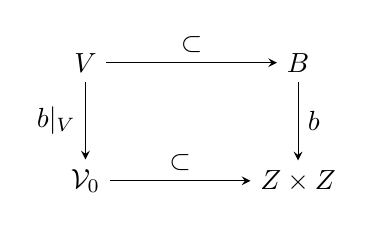
\begin{tikzpicture}[>=stealth, baseline=(current bounding box.center)]
\node (v) at (0,1.5) {$V$};
\node (b) at (2.7,1.5) {$B$};
\node (v0) at (0,0) {$\mathcal V_0$};
\node (zz) at (2.7,0) {$Z\times Z$};
\draw[->] (v)--node[above] {$\subset$} (b);
\draw[->] (v0)--node[above] {$\subset$} (zz);
\draw[->] (v)--node[left] {$b|_V$} (v0);
\draw[->] (b)--node[right] {$b$} (zz);
\end{tikzpicture}
\[
 \begin{gathered}
 V_z=\operatorname{Bl}_xX,\\
 (V\cap E)_z=\mathbb P(T_z^*D_\lambda)
       \subset E_z=\mathbb P(T_z^*Z).
 \end{gathered}
\]
\end{minipage}
\hfill
\begin{minipage}[c]{0.50\linewidth}
\centering
\small
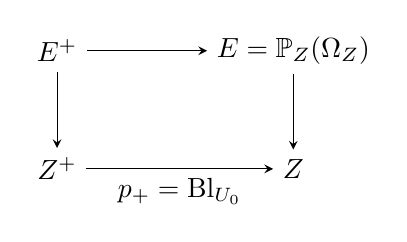
\begin{tikzpicture}[>=stealth, baseline=(current bounding box.center)]
\node (ep) at (0,1.5) {$E^+$};
\node (e) at (3,1.5) {$E=\mathbb P_Z(\Omega_Z)$};
\node (zp) at (0,0) {$Z^+$};
\node (z) at (3,0) {$Z$};
\draw[->] (ep)--(e);
\draw[->] (ep)--(zp);
\draw[->] (e)--(z);
\draw[->] (zp)--node[below] {$p_+=\operatorname{Bl}_{U_0}$} (z);
\end{tikzpicture}
\[
 \begin{gathered}
 J_+=p_+^{-1}(U_0),\qquad U_0=X\times\mathbb P^1,\\
 \mathcal J=(\mathcal I_V\cdot\cO_E)\cdot\cO_{E^+}.
 \end{gathered}
\]
\end{minipage}

\caption{Two geometric constructions used in the determinant estimate.
On the left, the strict transform \(V\subset B\) meets \(E_z\) in the
directions tangent to \(D_\lambda\).  Under the quotient convention,
the displayed projectivized cotangent spaces parametrize tangent lines.
On the right, \(E^+\) is the Cartesian base change
over \(Z^+=\operatorname{Bl}_{U_0}Z\), whose exceptional divisor is \(J_+\).
The restricted incidence ideal extends to \(\mathcal J\) on \(E^+\).
The ensuing local calculation identifies the normal parameter of \(J_+\)
among its generators.}
\label{zero:two-diagonals}
\end{figure}

The next lemma turns the pole bound in
Equation~\eqref{zero:pole-transfer} into a common vanishing order for the
coefficients of each determinant map.

\begin{lemma}\label{zero:determinant-order}
On a smooth projective modification \(h_+:U^+\to E^+\) one can choose
an approximation
\begin{equation}\label{zero:plus-decomposition}
 h_+^*(2p_+^*M+s\zeta)=\beta^++\{D^+\},
 \qquad \beta^+\ \text{Kähler},\quad D^+\ge0\ \text{rational},
\end{equation}
retaining the log-ideal orders of \(T|_E\), such that the general
fiber volume \(w^+\) of \(\beta^+\) over \(Z^+\) satisfies
\(w^+\ge w/2\).  Let \(f_+:U^+\to Z^+\) be the natural map and put
\[
 \Lambda^+=s h_+^*\cO_{E^+}(1)-\cO_{U^+}(D^+),\qquad
 \mathcal F_j^+=(f_+)_*\cO_{U^+}(j\Lambda^+),\qquad
 R_j^+=\operatorname{rk}\mathcal F_j^+ .
\]
For every sufficiently large divisible \(j\), write
\[
 \iota_j:\mathcal F_j^+\hookrightarrow p_+^*\operatorname{Sym}^{js}\Omega_Z,\qquad
 \varphi_j:\det\mathcal F_j^+\longrightarrow
       \bigwedge^{R_j^+}\!\bigl(p_+^*\operatorname{Sym}^{js}\Omega_Z\bigr)
\]
for the inclusion and its nonzero determinant map.  Here
\(\det\mathcal F_j^+=(\bigwedge^{R_j^+}\mathcal F_j^+)^{**}\), and the
determinant map extends across the complement of the locally free locus,
which has codimension at least two.
Localize a coordinate local ring of \(Z^+\) at the height-one prime of
\(J_+\), obtaining a discrete valuation ring \(R\) with uniformizer \(u\).
In local frames over \(R\), define
\[
 h_j=\min\{\operatorname{ord}_u(c):c\text{ is a nonzero coefficient of }\varphi_j\}.
\]
Equivalently, \(h_j\) is the minimum order of the maximal minors of
\(\iota_j\); it is independent of the frames.  If \(\sigma_{J_+}\) is the
canonical section of \(\cO_{Z^+}(J_+)\), then \(\varphi_j\) factors as
\[
 \det\mathcal F_j^+
 \xrightarrow{\ \cdot\sigma_{J_+}^{h_j}\ }
 \det\mathcal F_j^+(h_jJ_+)
 \xrightarrow{\ \widetilde\varphi_j\ }
 \bigwedge^{R_j^+}\!\bigl(p_+^*\operatorname{Sym}^{js}\Omega_Z\bigr),
\]
where \(\widetilde\varphi_j\) is holomorphic.  The common order satisfies
\begin{equation}\label{zero:determinant-order-equation}
 h_j\ge c_n\,jR_j^+s ,
\end{equation}
provided \(q\) is sufficiently large.
\end{lemma}

\begin{proof}
Blow up \(\mathcal J\) and take a common smooth projective resolution
with \(U\to E\) from Equation~\eqref{zero:selected-decomposition}.  Pull back
\(\beta\) and \(D'\).  Subtracting a sufficiently small rational
multiple of an effective exceptional divisor whose negative is
relatively ample makes the pulled-back Kähler class Kähler on this
resolution; add that multiple to the effective part.  Further upward
rational rounding may be
arbitrarily small.  This gives Equation~\eqref{zero:plus-decomposition} with all
original orders retained.  Its general fiber intersection is as close
to \(w\) as desired, so arrange \(w^+\ge w/2\).  Lemma~\ref{zero:direct-image}
and the effective divisor give
\begin{equation}\label{zero:plus-rank}
 \mathcal F_j^+\subseteq p_+^*\operatorname{Sym}^{js}\Omega_Z,\qquad
 R_j^+=\frac{w^+}{(d-1)!}j^{d-1}+O(j^{d-2}).
\end{equation}

We spell out the local order imposed on the polynomials in this
inclusion.  Near \(z=(x,x,\lambda)\), use coordinates
\((\mathbf x,\mathbf a,\lambda)\) on the first \(Z\), where \(\mathbf x\)
and \(\mathbf a\) each have \(n\) components and \(U_0=(\mathbf a=0)\).
Write the second coordinates as
\((\mathbf x+\mathbf h,\mathbf a+\mathbf k,\lambda+\mu)\), with
\(\mathbf h,\mathbf k\) each having \(n\)
components.  Then
\[
 \mathcal V_0=(\mathbf a=\mathbf k=\mu=0),\qquad
 \Delta_Z=(\mathbf h=\mathbf k=\mu=0).
\]
In a blowup chart meeting the lines tangent to \(D_\lambda\), take
\[
 h_1=v,\quad h_i=v\alpha_i\ (2\le i\le n),\quad
 k_i=vy_i\ (1\le i\le n),\quad \mu=vy_{n+1}.
\]
Here \(E=(v=0)\), while the strict transform is
\(V=(a_1=\cdots=a_n=y_1=\cdots=y_{n+1}=0)\).
In particular,
\begin{equation}\label{zero:ideal-before}
 \mathcal I_V|_E=(a_1,\ldots,a_n,y_1,\ldots,y_{n+1}).
\end{equation}
On a chart of the blowup of \(U_0\), write
\(a_1=u\) and \(a_i=u\tau_i\) for \(i\ge2\).  Along the general point
of \(J_+=(u=0)\), the ideal \(\mathcal J\) is exactly
\begin{equation}\label{zero:joint-ideal}
 (u,y_1,\ldots,y_{n+1}).
\end{equation}
Here \(u\) measures vanishing along \(J_+\), while the \(y_i\) measure
transverse fiber directions.  Thus a term of transverse degree \(\ell\)
can contribute at most \(\ell\) to the incidence order; the remaining
order must come from its coefficient in \(u\).  We now make this statement
precise.

Suppose locally that the singularities of \(T\) are
\(c\log|\mathfrak a|+O(1)\), with the logarithmic normalization for
which a divisorial coefficient is \(c\) times the ideal order.  If
\(k=\operatorname{ord}_V(\mathfrak a)\), then \(b_V=ck\).
The normal Taylor coefficients of degree less than \(k\) vanish on a
dense open set of \(V\), hence on \(V\) locally.  Thus
\(\mathfrak a\subseteq\mathcal I_V^k\) also near a general point of
\(V\cap E\).  Restricting to \(E\) and pulling to \(E^+\) gives the
corresponding order in Equation~\eqref{zero:joint-ideal}.  At its general center
the displayed generators are regular coordinates.  If \(H_{\mathcal J}\)
is the exceptional divisor of their blowup, its valuation is the
ordinary ideal-adic order:
\[
 \operatorname{ord}_{H_{\mathcal J}}(g)
  =\max\{k:g\in(u,y_1,\ldots,y_{n+1})^k\}.
\]
The common resolution dominates this blowup.  Pullback preserves the
effective difference between \(D'\) and the resolved log divisor,
and the later adjustments only increase the effective part.  Thus
\(D^+\) has coefficient at least \(b_V\) at this valuation.
Every polynomial image of a section of \(\mathcal F_j^+\) has
integral valuation at least \(\lceil jb_V\rceil\).  Locally bounded
remainders have zero order at this valuation.

There are \(n\) homogeneous coordinates along \(T_zD_\lambda\) and
\(n+1\) transverse homogeneous coordinates in \(T_zZ\).  Denote
these two groups by \(H_1,\ldots,H_n\) and
\(Y_1,\ldots,Y_{n+1}\).  For \(m=js\), a local polynomial in
\(\operatorname{Sym}^m(p_+^*\Omega_Z)\) has the form
\[
 \sum_{|\alpha|+|\gamma|=m}
          c_{\alpha,\gamma}(u)\,H^\alpha Y^\gamma.
\]
Work over the discrete valuation ring \(R\) used to define \(h_j\), choosing
the chart parameter \(u\) as uniformizer, and let \(\kappa\) be its residue
field.  The coefficients \(c_{\alpha,\gamma}\) lie in \(R\).
Equation~\eqref{zero:joint-ideal}
implies, monomial by monomial,
\begin{equation}\label{zero:coefficient-order}
 \operatorname{ord}_u(c_{\alpha,\gamma})
       \ge\max\{0,\lceil jb_V\rceil-|\gamma|\}.
\end{equation}
Indeed, on the chart \(H_1\ne0\), group the dehomogenized polynomial as
\[
 \sum_\gamma
 P_\gamma(H_2/H_1,\ldots,H_n/H_1)(Y/H_1)^\gamma,
 \qquad P_\gamma\in R[H_2/H_1,\ldots,H_n/H_1].
\]
Put \(b_j=\lceil jb_V\rceil\).  At the general center of
\((u,Y/H_1)\), order at least \(b_j\) forces
\(P_\gamma\) to be divisible by \(u^{b_j-|\gamma|}\) whenever
\(|\gamma|<b_j\).  Otherwise its first nonzero reduction would be a
nonzero polynomial over \(\kappa\), which stays nonzero in
\(\kappa(H_2/H_1,\ldots,H_n/H_1)\); in the associated graded ring
it would give a nonzero term of total \((u,Y/H_1)\)-degree less than
\(b_j\).  The transverse monomials there are independent.  Comparing
the internal polynomial coefficients over the base residue field
\(\kappa\) now gives Equation~\eqref{zero:coefficient-order}.

We compare the number of monomials with the rank estimate in
Equation~\eqref{zero:plus-rank}.  The
ambient rank and the number of monomials of transverse degree \(\ell\)
are
\[
 N_m=\binom{m+2n}{2n},\qquad
 N_{m,\ell}=\binom{\ell+n}{n}
             \binom{m-\ell+n-1}{n-1}.
\]
For fixed \(\delta\in(0,1)\), let \(H_m(\delta)\) count the monomials
with \(\ell>(1-\delta)m\).  Summing instead over their internal
degree gives
\[
 H_m(\delta)
 \le \binom{m+n}{n}\binom{\lceil\delta m\rceil+n}{n},\qquad
 \limsup_{m\to\infty}\frac{H_m(\delta)}{N_m}
       \le\binom{2n}{n}\delta^n.
\]
On the other hand, \(w^+\ge w/2\) and
Equation~\eqref{zero:plus-rank} show that the approximation on \(E^+\)
retains at least half the rank fraction in
Equation~\eqref{zero:selected-rank-fraction}:
\[
 \lim_{j\to\infty}\frac{R_j^+}{N_{js}}
       =\frac{w^+}{s^{d-1}}
       \ge\frac{w}{2s^{d-1}}\ge c_n>0.
\]
Fix \(\delta>0\), depending only on \(n\), so small that, for each fixed
\(q\) and its selected data, fewer than \(R_j^+/2\) monomials have transverse
degree greater than \((1-\delta)js\) for all sufficiently large divisible
\(j\).  For each
remaining monomial, Equation~\eqref{zero:coefficient-order} and
Lemma~\ref{zero:incidence-pole} give
\[
 \operatorname{ord}_u(c_{\alpha,\gamma})
   \ge j(s-C_n)-(1-\delta)js
   =j(\delta s-C_n)\ge\frac{\delta js}{2}.
\]
The last inequality holds once \(q\) is large, since
\(s\ge c_nA_q\to\infty\).

Over the same discrete valuation ring \(R\), the torsion-free sheaf
\(\mathcal F_j^+\) becomes a free module of rank \(R_j^+\).  Write its
inclusion into the symmetric power as a matrix with the monomials
as rows.  Every maximal minor uses at least \(R_j^+/2\) of the rows
whose coefficients have order at least \(\delta js/2\).  All maximal
minors therefore have order at least
\(\delta jR_j^+s/4\).  By the definition of \(h_j\), this proves
Equation~\eqref{zero:determinant-order-equation}.  Dividing the determinant
map by \(\sigma_{J_+}^{h_j}\) gives a holomorphic map at every point of
codimension one: the coefficients have the required order along \(J_+\),
and its local equation is a unit away from \(J_+\).  Hartogs' theorem
extends the divided map across the remaining set of codimension at least
two, giving the stated factorization through
\(\det\mathcal F_j^+(h_jJ_+)\).
\end{proof}

\subsubsection{Cancellation on the point blowup}

\begin{proof}[Completion of the proof of Proposition~\ref{zero:line-nonvanishing}]
Fix \(q\) sufficiently large for the preceding lemmas, with its chosen
\(P,s,T\) and modifications.  Choose a very general point \(x\) in the first
factor of \(X^2\).  The slice of \(Z^+\) above \(x\) is
\[
 S=\mathbb{P}_Y(\cO_Y\oplus a^*\mathscr L),\qquad
 a:Y=\operatorname{Bl}_xX\longrightarrow X,
\]
and \(J_+|_S\) is the pullback of \(F\).  We choose \(x\) so that
Equation~\eqref{zero:slope-blowup}, Equation~\eqref{zero:point-bound}, the restrictions of
the currents below, and all determinant maps for divisible \(j\)
can be tested on this slice.  These exclude at most countably many
proper analytic sets and the measure-zero exceptional sets for
current restrictions.

Write the restricted determinant line as
\[
 (\det\mathcal F_j^+)|_S
   =\pi_S^*\mathscr Q_j^+\otimes\cO_S(\ell_j^+),\qquad
 Q_j^+=c_1(\mathscr Q_j^+).
\]
Factoring the common zero of order \(h_j\) from the determinant
map gives a nonzero map whose source on \(S\) is
\[
 \pi_S^*(\mathscr Q_j^+\otimes\cO_Y(h_jF))
                 \otimes\cO_S(\ell_j^+).
\]
The plus sign of \(h_jF\) follows because division of the map by
the local equation of \(J_+^{h_j}\) enlarges its source from
\(\det\mathcal F_j^+\) to
\(\det\mathcal F_j^+\otimes\cO(h_jJ_+)\).
Its target embeds into the \(jsR_j^+\)-fold tensor of the
restriction of \(p_+^*\Omega_Z\).  In particular we use the
cotangent bundle of the original \(Z\), with its restricted
filtration
\[
 0\longrightarrow
 \pi_S^*(\cO_Y^{\oplus n}\oplus a^*\Omega_X)
 \longrightarrow (p_+^*\Omega_Z)|_S
 \longrightarrow
 \cO_S(-2)\otimes\pi_S^*a^*\mathscr L
 \longrightarrow0.
\]
The same homogeneous-monomial calculation as in
Equation~\eqref{zero:determinant-bound-Z}, now applying
Equation~\eqref{zero:slope-blowup} to the second factor of \(X^2\), gives
\begin{equation}\label{zero:determinant-bound-slice}
 \ell_j^+\le0,\qquad
 Q_j^++h_j\{F\}
       \le(jsR_j^+-\ell_j^+)a^*L.
\end{equation}
More explicitly, if the chosen graded term has \(i\) relative
factors, the pushed polynomial has degree
\(-2i-\ell_j^+\ge0\).  Its exponent in \(a^*\mathscr L\), together
with the \(i\) relative factors and the cotangent order from the second
factor of \(X^2\), is at most \(jsR_j^+-\ell_j^+\).  The cotangent
factors from the first factor of \(X^2\) are constant.  This proves the
displayed inequality using
the tensors of \(a^*\Omega_X\), without introducing \(\Omega_Y\)
or \(\Omega_{Z^+}\).

Apply Lemma~\ref{zero:direct-image} to the decomposition in
Equation~\eqref{zero:plus-decomposition}.  Equation~\eqref{zero:GRR-base}
shows that the limits of the restricted determinant components divided by
\(jR_j^+\) exist; denote them by \(Q^+\) and \(\ell^+\).  Divide
Equation~\eqref{zero:determinant-bound-slice} by \(jR_j^+\), use
Equation~\eqref{zero:determinant-order-equation}, and pass to the closed
pseudo-effective cone.  We obtain
\begin{equation}\label{zero:slice-upper}
 \ell^+\le0,\qquad
 Q^++c_ns\{F\}\le(s-\ell^+)a^*L.
\end{equation}
The pseudo-effective class in Equation~\eqref{zero:GRR-base}, restricted to the
very general slice \(S\), is
\begin{equation}\label{zero:slice-psef}
 \pi_S^*(Q^++2a^*P)+(\ell^++2q)\xi\ge0.
\end{equation}
Testing on a general vertical line gives \(\ell^++2q\ge0\).
Let \(A\subset S\) be the axis of
\(\mathbb{P}_Y(\cO_Y\oplus a^*\mathscr L)\) with divisor class \(\{A\}=\xi\).
On \(A\simeq Y\), its normal class is \(\{A\}|_A=\xi|_A=a^*L\ge0\).
Add an arbitrarily small Kähler class to the class in
Equation~\eqref{zero:slice-psef}, and choose a Kähler current with analytic
singularities in the resulting big class.  Remove its generic divisorial
pole along \(A\) and restrict
the residual current to \(A\).  Adding back the removed nonnegative multiple
of \(a^*L\) preserves pseudo-effectivity.  Passing to the limit gives
\begin{equation}\label{zero:slice-lower}
 Q^++2a^*P+(\ell^++2q)a^*L\ge0.
\end{equation}

The slope bound in Equation~\eqref{zero:slice-upper} supplies the
pseudo-effective class \((s-\ell^+)a^*L-Q^+-c_ns\{F\}\).  Adding it to
Equation~\eqref{zero:slice-lower} cancels the entire normalized determinant
class restricted to the axis, \(Q^++\ell^+a^*L\), leaving
\[
 2a^*P+(s+2q)a^*L-c_ns\{F\}\ge0.
\]
Since \(L\le P/r\), the point bound in Equation~\eqref{zero:point-bound} implies
\begin{equation}\label{zero:contradiction}
 \frac{c_ns}{\,2+(s+2q)/r\,}\le C_n.
\end{equation}
The denominator is bounded independently of \(q\), because
\(s\le C_nq^{1/d}\) and \(r\ge q^2\).  The numerator tends to
infinity, because \(s\ge c_nq^{1/d}\).  Equation~\eqref{zero:contradiction}
is impossible for arbitrarily large \(q\).

For each \(q\), the choice of \(t(q)\), the rational \(s\), the current
\(T\), and the modifications precedes the limit in \(j\).  The monomial
cutoff \(\delta\) depends only on \(n\), while the required lower bound for
divisible \(j\) may depend on the fixed data.  We choose the very general
points after those data are fixed.
Thus every simultaneous general-point test above involves at most
countably many conditions, and no bound depends on the point.
The contradiction disproves the contrary hypothesis and proves
Proposition~\ref{zero:line-nonvanishing}.
\end{proof}

\subsection{Vanishing on the simple model}

We now apply Proposition~\ref{zero:line-nonvanishing} to the sum of
the canonical bundle and the nef line bundle whose class we wish to
eliminate.  The remaining use of the ordinary adjoint
decomposition is particularly short: it turns meromorphic
nonvanishing into both signs of pseudo-effectivity.

\begin{proposition}\label{zero:simple-vanishing}
Let \(X\) be a smooth simple compact Kähler manifold of algebraic
dimension zero carrying a generically nondegenerate holomorphic
two-form.  Every nef rational holomorphic line bundle on \(X\) has zero
first Chern class.
\end{proposition}

\begin{proof}
The assertion is immediate for a point.  A positive-dimensional space
of algebraic dimension zero cannot be a curve, so assume \(\dim X\ge2\).
If \(q(X)>0\), its Albanese map is generically finite onto its image,
by simplicity.  Ueno's structure theorem for subvarieties of complex
tori makes this image a translate of a torus: its quotient by the
connected stabilizer is of general type, and positive dimension of that
quotient would contradict algebraic dimension zero \cite{Ueno}.
Lemma~\ref{zero:mass-test} proves the conclusion.

The same argument applies after any smooth generically finite Kähler
cover of \(X\) having positive irregularity.  Such a cover is still
simple and has algebraic dimension zero; vanishing upstairs descends
by push--pull.  We may therefore suppose that every such cover has
irregularity zero.  Lemma~\ref{zero:no-correspondences} then describes
the subvarieties through a very general point of \(X^2\).

Clear denominators and let \(N_0\) be the resulting nef holomorphic line
bundle.  A top wedge of the generically nondegenerate two-form is a
nonzero holomorphic section of \(K_X\).  In particular \(K_X\) is
effective.  Set
\[
 \mathscr L=K_X+N_0,\qquad L=c_1(\mathscr L).
\]
The class \(L\) is pseudo-effective and dominates \(c_1(K_X)\).
Lemma~\ref{zero:cotangent-slope} supplies both slope inequalities.
Every hypothesis of Proposition~\ref{zero:line-nonvanishing} is now
satisfied.  Some positive power of \(K_X+N_0\) therefore has a nonzero
meromorphic section.  Dividing by the corresponding power of a
canonical section shows that \(N_0\), as a rational line bundle, is
represented by a signed divisor.

Resolve its positive and negative parts.  On the resulting smooth
Kähler model write
\[
 N_0\qsim E-G,\qquad E,G\ge0,
\]
with rational coefficients and simple normal crossing union of their
supports; we suppress the pullback notation for \(N_0\).  The canonical
bundle \(K'\) of this model remains effective.  Choose a small rational
\(u>0\) so that both \(uE\) and \(uG\) are klt boundaries.
The ordinary decomposition, Theorem~\ref{pre:ordinary}, applies to
\(K'+uE\) and \(K'+uG\).  On a common higher model, denote their pulled
back classes by \(\alpha_E\) and \(\alpha_G\).  Algebraic dimension zero
makes each semiample part rationally trivial, so that the pulled back
rational lines equal their negative divisors.  Since
\(\alpha_E-\alpha_G=u\{N_0\}\) is nef,
Lemma~\ref{pre:negative}\,(2) gives
\[
 N(\alpha_E)\le N(\alpha_G),\qquad
 u\{N_0\}=\{N(\alpha_E)-N(\alpha_G)\}.
\]
Thus \(-\{N_0\}\) is pseudo-effective, whereas \(\{N_0\}\) is nef.
Pairing both classes with a Kähler power gives zero mass, and hence
\(\{N_0\}=0\).  Pullback injectivity yields the same conclusion on
\(X\).
\end{proof}

\begin{proof}[Proof of Proposition~\ref{zero:vanishing}]
Lemma~\ref{zero:geometric-reduction} reduces the assertion to
Proposition~\ref{zero:simple-vanishing}, which proves it.
In particular, once the induction has reached dimension \(n\), the
ordinary decomposition of \(K_T+B\) also proves the decomposition
assertion of Theorem~\ref{thm:decomposition} in algebraic dimension
zero: adding the nef line changes no Chern class.  Its semiample positive
part is rationally trivial, and its negative part is unchanged.
\end{proof}

\section{The nef summand on the algebraic-reduction fibers}
\label{sec:cycles}

Let $T$ be a smooth compact K\"ahler manifold of dimension $n$, and suppose
that $0<a(T)<n$.  After resolving its algebraic reduction, we have a
fibration $h:T\to W$ with $W$ smooth projective.  The objective of this
section is to show that a nef rational line bundle $M$ occurring in the
adjoint decomposition theorem has numerically trivial restriction to a
general fiber of $h$.  Proposition~\ref{desc:nef} will then descend its
class to $W$, after modifications.

The inductive decomposition on an individual fiber supplies a semiample
positive part only up to a flat twist.  To obtain sections on the total
space, we must choose the twists from a countable collection of global
line bundles.  Relative divisor cycles provide the required countable
collection of maps.  We first isolate the two ingredients of this
construction.

\subsection{Sections and coherent base change}

\begin{lemma}\label{cycle:sections}
Let $h:X\to W$ be a holomorphic algebraic reduction of a smooth connected
compact complex manifold, with connected fibers and smooth projective
base.  Let $(L_i)_{i\in I}$ be a countable collection of rational
holomorphic line bundles on $X$.  Outside a countable union of nowhere
dense subsets of $W$, a smooth fiber $F$ of $h$ satisfies
\[
                         \kappa(F,L_i|_F)\leq 0
                         \qquad\text{for every }i\in I.
\]
Any prescribed countable collection of further conditions holding on
dense open subsets of $W$ can be imposed on the same fiber.
\end{lemma}

\begin{proof}
Choose a positive integer $q_i$ such that $q_iL_i$ is an actual line
bundle.  For every positive multiple $m$ of $q_i$, the proper direct-image
theorem gives a coherent analytic sheaf
\[
                         \mathcal E_{i,m}=h_*\cO_X(mL_i)
\]
on $W$.  Work over the smooth-fibration locus, where the line bundle
is flat over the base.  On a dense open set where the dimension of
fiberwise sections is locally constant, coherent base change gives
the isomorphism
\begin{equation}\label{cycle:base-change}
 \mathcal E_{i,m}\otimes\C(w)
       \simeq H^0(X_w,\cO_{X_w}(mL_i|_{X_w}))
\end{equation}
by \cite[Section~7, Satz~5]{Grauert}.  It suffices here
to delete proper analytic subsets within dense open sets of $W$.
Fix an ample line bundle $H$ on $W$.  By GAGA and Serre's theorem,
$\mathcal E_{i,m}\otimes H^{k_{i,m}}$ is generated by global sections for
some integer $k_{i,m}$.  The projection formula and
\eqref{cycle:base-change} therefore show that all sections of
$mL_i|_{X_w}$ lift, after choosing a nonzero frame of $H^{k_{i,m}}$ at
$w$, to global sections of
\[
                    \cO_X(mL_i)\otimes h^*H^{k_{i,m}}.
\]

There are only countably many pairs $(i,m)$.  Choose $w$ in the smooth
locus of $h$, outside all the base-change exceptions and the further
generic exceptions in the statement.  If
$\kappa(X_w,L_i|_{X_w})>0$, some divisible $m$ has two sections whose
ratio is nonconstant on the connected fiber $X_w$.  Lifting these
sections as above gives a meromorphic function on $X$ whose restriction
to $X_w$ is that ratio.  Every meromorphic function on $X$ factors
through its algebraic reduction.  Such a function, when defined on a
nonempty open subset of the smooth fiber $X_w$, is constant there:
a local holomorphic section of $h$ through a point where the quotient
is holomorphic shows that the base function extends holomorphically
at $w$.  This contradicts the chosen nonconstant ratio.

The countable simultaneous choice is legitimate by Baire's theorem.
If a generic assertion is initially established on a dense open set,
a proper analytic exceptional subset of that open is still nowhere
dense in $W$.  Thus such generic assertions can also be included in the
choice.
\end{proof}

\subsection{Divisor incidence and a countable collection of fibrations}

We use the cycle-space results of Barlet, Lieberman, and Fujiki
\cite{Barlet,LiebermanCycles,Fujiki1978,Fujiki}.  In the form needed here,
the spaces of
effective cycles of a compact K\"ahler manifold have countably many
irreducible components; each component is compact and belongs to
Fujiki's class $\mathcal C$; see \cite[p.~189]{Fujiki}.  The locus of
cycles contained in a fiber of a proper map is an analytic relative
cycle space \cite[Proposition~3.2]{Fujiki1978}.  We also use the
meromorphic fiber map obtained by analytic flattening: after modifying
the base, the flat strict transform has an analytic family of fiber
cycles and hence a holomorphic map to the cycle space
\cite[Chapter~V]{Barlet}.  All parameter spaces and images in class $\mathcal C$
will be replaced by smooth compact K\"ahler models when needed.

The following observation explains why the numerical class of a divisor
can detect a semiample fibration without fixing its flat twist.

\begin{lemma}\label{cycle:divisors}
Let $F$ be a smooth connected compact K\"ahler manifold, let $A$ be a
rational line bundle on $F$, and suppose that a modification
$\rho:\widehat F\to F$ from a smooth compact K\"ahler manifold satisfies
\begin{equation}\label{cycle:fiber-decomposition}
 \rho^*A\num P+R,
 \qquad P\text{ semiample},
 \qquad R=N(c_1(\rho^*A))\text{ a rational divisor}.
\end{equation}
Let $g:\widehat F\to Q$ be the fibration defined by $P$, so that $Q$ is
normal projective and $P\qsim g^*H_Q$ for an ample rational line bundle
$H_Q$.  There is a dense open subset $U\subset F$, independent of the
divisors below, with the following properties for every sufficiently
divisible positive integer $m$.
\begin{enumerate}
\item There exists an analytic family of effective
divisors on $F$ with class $m c_1(A)$ that distinguishes the general fibers
of the meromorphic fibration $g\circ\rho^{-1}$.
\item For every effective divisor $D$ with class
$m c_1(A)$, membership
in $\operatorname{Supp}D$ is constant along the intersection of $U$
with a general smooth fiber of that meromorphic fibration.
\end{enumerate}
\end{lemma}

\begin{proof}
The difference between the two sides of
\eqref{cycle:fiber-decomposition} is flat as a rational line bundle.
By Lemma~\ref{pre:picard}, there is a flat rational line
bundle $\eta$ on $F$ such that
\[
                         \rho^*(A+\eta)\qsim P+R.
\]
Choose $m$ clearing the denominators and such that $mH_Q$ is very ample.
The divisors
\[
                   g^*D_Q+mR,
                   \qquad D_Q\in|mH_Q|,
\]
descend to an analytic family of divisors on $F$ with class $m c_1(A)$.
Indeed $\rho_*\cO_{\widehat F}=\cO_F$, so the projection formula
identifies sections of $m(A+\eta)$ with sections of its pullback.
On the isomorphism locus of $\rho$, away from $\operatorname{Supp}R$,
they distinguish general $g$-fibers, since hyperplanes distinguish
points of $Q$.

For an arbitrary effective divisor $D$ of this class,
Lemma~\ref{pre:negative}(1) gives
\[
                         \rho^*D\geq mR.
\]
The residual divisor $D'=\rho^*D-mR$ is effective and has class
$m c_1(P)$.  Let $G$ be a smooth compact connected fiber of $g$.  If
$D'$ does not contain $G$, its restriction is an effective divisor of
class zero on $G$, hence is empty: in positive dimension this follows
by integrating against a K\"ahler form to the appropriate power.
Consequently $\operatorname{Supp}D'$ either contains $G$ or misses it.
For a point fiber the same alternative is immediate.  Taking the image
of the isomorphism locus of $\rho$, and deleting
$\operatorname{Supp}R$ and the nonsmooth locus of $g$, gives the stated
open set $U$.  This choice uses only $\rho$, $R$, and $g$, and works for
all the divisors simultaneously.
\end{proof}

\begin{lemma}\label{cycle:detection}
Let $h:X\to W$ be a fibration of smooth connected compact K\"ahler
manifolds with $\dim W<\dim X$, and let $A$ be a rational line bundle
on $X$.  There is a countable collection of diagrams
\begin{equation}\label{cycle:diagrams}
 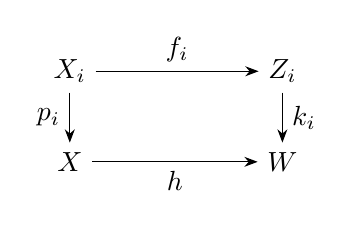
\begin{tikzpicture}[baseline=(current bounding box.center),>=Stealth]
 \node (Xi) at (0,1.15) {$X_i$};
 \node (Zi) at (2.7,1.15) {$Z_i$};
 \node (X) at (0,0) {$X$};
 \node (W) at (2.7,0) {$W$};
 \draw[->] (Xi) -- node[above] {$f_i$} (Zi);
 \draw[->] (Xi) -- node[left] {$p_i$} (X);
 \draw[->] (Zi) -- node[right] {$k_i$} (W);
 \draw[->] (X) -- node[below] {$h$} (W);
 \end{tikzpicture}
\end{equation}
where $p_i$ is a modification, $f_i$ is a fibration, and $X_i,Z_i$ are
smooth compact K\"ahler manifolds, with the following property.

For a very general smooth fiber $F=X_w$, suppose that a smooth compact
K\"ahler modification $\rho:\widehat F\to F$ has a decomposition
\eqref{cycle:fiber-decomposition} for $A|_F$, and that the fibration
$g:\widehat F\to Q$ defined by $P$ has positive-dimensional base.
For some $i$, the restriction of $f_i$ over $w$ is bimeromorphically
equivalent to $g$.  In particular, on a common resolution, their
general fibers coincide.  The collection and the exceptional subsets
of $W$ can be fixed before $F$, $\rho$, $P$, and $R$ are chosen.
\end{lemma}

\begin{proof}
We associate a map to each component of the relative divisor space by
recording all its divisors through a point.  On a fiber with the stated
decomposition, Lemma~\ref{cycle:divisors} makes these incidence supports
constant along the semiample fibration.  Integral multiplicities will
then give constancy of the cycle maps themselves, while the
distinguishing linear system will give the converse.

Put $d=\dim X-\dim W$, and let $W^\circ$ be the smooth-fibration locus
of $h$.  Consider the relative cycle spaces whose points are pairs
$(w,D)$, where $D$ is an effective $(d-1)$-cycle in $X_w$.  They are
closed subspaces of the product of $W$ with the corresponding compact
cycle components of $X$.  Thus they have countably many compact
irreducible components in class $\mathcal C$.

For each positive integer $m$ clearing the denominator of $A$, retain
the components meeting $W^\circ$ on which the divisor class is
$m c_1(A|_{X_w})$.  This is a condition on an entire component over
$W^\circ$: in a smooth family the cohomology class of an analytic
family of cycles is locally constant, and $c_1(A)$ supplies a global
section of the same cohomology local system.  After resolving a
component, its open part over $W^\circ$ is connected, so equality at
one point implies equality throughout that part.  Components not
dominating $W$ have proper analytic images; exclude all these images
from the eventual choice of $w$.

Fix a retained dominating component and a smooth compact K\"ahler
resolution $S$ of it.  Denote its divisor at $s\in S$ by $D_s$ and form
the incidence
\[
                    \mathcal I_S
                       =\{(x,s)\in X\times S:x\in\operatorname{Supp}D_s\}.
\]
We take the incidence of the analytic cycle family, including its
limits from the open part over $W^\circ$.  Over that open part it is a
family of pure $(d-1)$-dimensional cycles.  Hence every irreducible
component there dominates $S$ and has dimension $\dim S+d-1$.
Let $I_1,\ldots,I_t$ be the incidence components that dominate $X$.
The other components have proper analytic images in $X$; outside
those images they contribute nothing to incidence.

For each $I_j\to X$, analytic flattening gives a meromorphic map
recording its generic fiber as an effective cycle in $S$.  All these
cycles have dimension
\[
                         e=\dim S+d-1-\dim X.
\]
Taking the tuple of these maps, together with $h$, gives a meromorphic
map $\Phi_S$ from $X$ into $W$ times a finite product of compact cycle
components of $S$.  On a dense open subset of $X$, the union of the
supports of the recorded cycles is precisely
\begin{equation}\label{cycle:incidence-support}
                         \{s\in S:x\in\operatorname{Supp}D_s\}.
\end{equation}
In obtaining this open set we discard the images of the nondominating
incidence components and the exceptional sets of the fiber maps.
The target components and the image of $\Phi_S$ belong to class
$\mathcal C$.  Resolving the graph, taking Stein factorization, and
replacing the base by a smooth compact K\"ahler model therefore gives
a diagram \eqref{cycle:diagrams}.  The coordinate $h$ ensures that its
base maps to $W$.  If there is no dominating incidence component, we
retain only the coordinate $h$; such a component will not be needed
to detect a positive-dimensional $Q$.

This construction gives countably many diagrams.  Fix their models,
their incidence-recording open sets, and their Stein factorizations.
We may simultaneously require that their fibers over the eventual
$w$ be smooth, that $p_i$ restrict to a modification over $w$, and that
each of the dense open sets used meet the corresponding fiber densely.
For any one diagram these are generic conditions, by properness,
generic smoothness, and the fiber-dimension theorem.  In particular,
let $U_i\subset Z_i$ be the locus over which $f_i$ is smooth.  We
require that $k_i^{-1}(w)$ meet $U_i$ densely.  To justify this
condition, a component of $Z_i\setminus U_i$ that does not dominate
$W$ has proper image, whereas a component dominating $W$ has general
fiber of dimension strictly less than $\dim Z_i-\dim W$.
Since the general $k_i$-fiber is smooth of that pure dimension, it
cannot have a component contained in $Z_i\setminus U_i$.  The same
conditions may be imposed after any preselected countable collection
of further modifications of these diagrams.

We now choose such a very general $w$ and a decomposition on $F=X_w$
as in the statement.  By Lemma~\ref{cycle:divisors}, a projective
linear system of divisors of class $m c_1(A|_F)$ distinguishes the
general $g$-fibers for some $m$.  Its image in the relative cycle
space is irreducible and lies in one irreducible component.  That
component dominates $W$, since all images of nondominating components
were excluded.  It is therefore one of the components used above.
Passing to its parameter resolution $S$ preserves the distinguishing
property: every divisor still has a preimage in $S$.

The map $\Phi_S|_F$ distinguishes general $g$-fibers.  Indeed two
different general points of $Q$ are separated by a divisor in the
chosen linear system, so their incidence supports
\eqref{cycle:incidence-support} differ.  Conversely, fix a general
smooth connected $g$-fiber $G$.  On the common open set of
Lemma~\ref{cycle:divisors} and the incidence recording, membership in
every divisor $D_s$ is constant along $G$.  Thus the support in
\eqref{cycle:incidence-support} is fixed as the point moves in that
open part of $G$.

This support assertion also gives constancy of the recorded
\emph{cycles}.  Their fixed union of supports is pure $e$-dimensional
and has finitely many irreducible components.  Since all recorded
cycles have dimension $e$, there are only countably many possible tuples of
effective cycles supported there: their multiplicities are
nonnegative integers.  A holomorphic map from a connected complex
manifold with countable image is constant.  Removing a proper
analytic subset from the smooth connected $G$ leaves a connected
open set, so $\Phi_S$ is constant on a general $g$-fiber.  Point
fibers require no separate argument.

Constancy on the general connected fibers gives a meromorphic
factorization through $Q$.  One can see this by taking the image of
the graph in $Q$ times the target: its projection to $Q$ has one-point
general fibers and is bimeromorphic.  The distinguishing property
makes the induced map from $Q$ generically one-to-one onto its image.
Hence $\Phi_S|_F$ defines the same meromorphic fibration as $g$.

Finally, the restriction of $f_i$ over $w$ still has connected fibers:
its fibers are exactly the corresponding fibers of $f_i$.  Its base
over $w$ is connected, being the image of the connected source fiber.
The finite map in Stein factorization cannot split a connected
general $g$-fiber: a map from that fiber into a finite set is constant.
The preselected resolutions restrict to modifications over $w$.
Thus the same comparison holds for $f_i$, proving the assertion.
\end{proof}

\subsection{Vanishing of the nef class on the fibers}

We can now choose the flat twists on the total space.  The order of
choice is essential: the following proof fixes a countable collection
of global representatives before it chooses the smooth fiber.

\begin{proposition}\label{cycle:nef-summand}
Assume Theorem~\ref{thm:decomposition} in dimensions less than $n$.
Let $T$ be a smooth connected compact K\"ahler $n$-fold with
$0<a(T)<n$, and let $h:T\to W$ be a holomorphic algebraic reduction
with smooth projective base and connected fibers.  Let $B$ be an
effective rational SNC divisor with coefficients less than one,
assume that $J=K_T+B$ is pseudo-effective, and let $M$ be a nef
rational line bundle.  Then
\[
                              c_1(M|_F)=0
\]
for a general smooth fiber $F$ of $h$.
\end{proposition}

\begin{proof}
Set $A=J+M$.  By Theorem~\ref{pre:ordinary}, fix an effective rational
divisor $E$ with $J\qsim E$.  Apply Lemma~\ref{cycle:detection} to $h$
and $A$, and
fix its countable collection $(p_i,f_i,k_i)$.  Let $I_0$ be the subset
of indices for which $c_1(p_i^*M)$ vanishes on the general smooth
fiber of $f_i$.  For every $i\in I_0$, apply
Corollary~\ref{desc:representative} to $p_i^*M$ on $X_i$.  It gives a
representative on $X_i$ differing from $p_i^*M$ by a flat rational
line.  By Lemma~\ref{pre:picard}(2), that flat difference comes from
$T$.  We therefore obtain a rational line bundle $M_i^*$ on $T$, with
\[
                              M_i^*\num M,
\]
whose pullback is an actual rational pullback from the intermediate
base, after further modifications of the diagram.  Fix one such
representative and one such diagram for every $i\in I_0$.  In
particular, $M_i^*$ restricts rationally trivially to a general fiber
of that modified fibration.  This is a countable collection of
choices on $T$.

Choose $w\in W$ simultaneously satisfying the detection lemma and
its generic conditions for all the further diagrams just fixed.
Require also the conclusion of Lemma~\ref{cycle:sections} for the
countable collection
\[
                              (J+M_i^*)_{i\in I_0}.
\]
We take $F=T_w$ smooth, with $B|_F$ an SNC klt boundary.
We also require that the defining section of $E$ restrict
nontrivially to $F$; then
\[
                       J_F:=K_F+B|_F\qsim E_F:=E|_F\geq0.
\]
All the choices preceding $w$ depend only on data on the total space.

Suppose, towards a contradiction, that $M|_F\not\num0$.  The
lower-dimensional decomposition theorem gives a modification
$\rho:\widehat F\to F$ and
\begin{equation}\label{cycle:inductive-decomposition}
 \rho^*(J_F+M|_F)\num P_F+R_F,
 \qquad R_F=N(c_1(\rho^*(J_F+M|_F))),
\end{equation}
where $P_F$ is semiample and $R_F$ is a rational effective divisor.
Lemma~\ref{pre:negative}, applied to the nef summand $\rho^*(M|_F)$,
gives
\begin{equation}\label{cycle:residual-effective}
 R_F\leq N(c_1(\rho^*J_F))\leq\rho^*E_F,
 \qquad
 P_F\num(\rho^*E_F-R_F)+\rho^*(M|_F).
\end{equation}
Let $g:\widehat F\to Q$ be the fibration defined by $P_F$.  If
$Q$ were a point, the last equality would make a nef class and an
effective divisor sum to zero.  Pairing with a K\"ahler power would
give $\rho^*(M|_F)\num0$, contrary to the assumption.  Hence
$\dim Q>0$.

On a general smooth $g$-fiber $G$, the class of $P_F$ is zero.
Restricting the last equality in
\eqref{cycle:residual-effective} and using the same positivity
argument shows that
\begin{equation}\label{cycle:restriction-zero}
 c_1(\rho^*(M|_F)|_G)=0,
 \qquad
 G\cap\operatorname{Supp}(\rho^*E_F-R_F)=\varnothing.
\end{equation}
If $G$ is a point, the first assertion is automatic and the second
holds for a general point.  In positive dimension, choose a general
fiber not contained in the effective divisor, restrict it, and
integrate the effective and nef classes against a K\"ahler power.
Both nonnegative masses must vanish.

Lemma~\ref{cycle:detection} gives an index $i$ such that the restriction
of $f_i$ over $w$ and $g$ have the same general fibers up to modifications.  By
\eqref{cycle:restriction-zero} and injectivity of pullback on
cohomology, $p_i^*M$ has class zero on a smooth $f_i$-fiber above
$w$.  Such a fiber can be chosen in the smooth-fibration locus of
$f_i$, by the generic conditions already imposed.  Over the
connected smooth locus in $Z_i$, the restrictions of this Chern
class form a locally constant section of $R^2(f_i)_*\R$.  Vanishing
at one fiber therefore implies vanishing at every fiber in this
locus.  Thus $i\in I_0$; its representative $M_i^*$ was already
chosen before $w$.

We claim that
\begin{equation}\label{cycle:positive-kappa}
                         \kappa(F,J_F+M_i^*|_F)>0.
\end{equation}
On a common resolution of the maps on $F$, the line $M_i^*|_F$
is rationally trivial on a general $g$-fiber because it is a
pullback from the intermediate base of $f_i$.  This triviality
descends between smooth models of the fiber: for a modification,
pullback on line bundles is injective by normality and the
projection formula.  The difference
\[
             \Lambda=\rho^*(J_F+M_i^*|_F)-P_F-R_F
\]
is a flat rational line bundle by
\eqref{cycle:inductive-decomposition}.  Its restriction to a
general $G$ is rationally trivial.  Indeed $P_F|_G$ is trivial,
$M_i^*|_G$ is trivial, and
\eqref{cycle:restriction-zero} makes
$\cO_{\widehat F}(\rho^*E_F-R_F)|_G$ trivial, while
$J_F\qsim E_F$.

Resolve $Q$ and the induced map, and continue to denote the
resulting fibration between smooth models by $g$.  By Lemma~\ref{desc:flat},
$\Lambda\qsim g^*\lambda$ for a flat rational line bundle
$\lambda$ on the smooth projective base.  The line $P_F$ is the
pullback of the ample rational line on the original $Q$; on its
resolution the corresponding base line $H_Q'$ is nef and big.
Twisting by $\lambda$ preserves bigness.  On these models we have
an actual rational identity
\[
                \rho^*(J_F+M_i^*|_F)
                        \qsim g^*(H_Q'+\lambda)+R_F.
\]
Multiplication by the canonical section of a divisible multiple
of $R_F$ embeds the section spaces of the big base line into the
section spaces on $\widehat F$.  Since $\dim Q>0$, this proves
\eqref{cycle:positive-kappa}.

This contradicts the instance of Lemma~\ref{cycle:sections} imposed
on $J+M_i^*$ when $w$ was chosen.  Hence $M|_F\num0$ for the
chosen fiber.  Finally, restrictions of $c_1(M)$ form a
locally constant section of $R^2h_*\R$ on the connected smooth
locus of $h$.  Their vanishing therefore holds on every fiber in
that locus, and in particular on a general smooth fiber.
\end{proof}

\begin{corollary}\label{cycle:base-descent}
Under the assumptions of Proposition~\ref{cycle:nef-summand},
there are modifications $p:T'\to T$ and $b:W'\to W$, with
$T'$ smooth compact K\"ahler and $W'$ smooth projective, a
fibration $h':T'\to W'$ lifting $h$, and a nef rational line
bundle $N$ on $W'$ such that
\[
                              p^*M\num(h')^*N.
\]
\end{corollary}

\begin{proof}
Proposition~\ref{cycle:nef-summand} supplies the fiberwise
vanishing required in Proposition~\ref{desc:nef}.  Apply that
proposition to $h$ and $M$.  The modified base remains projective,
so the descended rational class is nef.
\end{proof}

\section{Completion of the induction}\label{sec:completion}

We now combine the preceding constructions. The main geometric step is
to make the ordinary adjoint semiample after adding a sufficiently
positive line from the algebraic base, while preserving the map to that
base. The adjoint formula of Proposition~\ref{adj:base} then puts the
problem on a projective variety. We first isolate the negative-part
calculation needed to pull the projective answer back.

\subsection{Divisors above subsets of codimension at least two}

\begin{lemma}\label{finish:exceptional}
Let \(r:V\to S\) be a surjective morphism from a smooth compact K\"ahler
manifold to a normal projective variety. Let \(H\) be a nef rational
Cartier divisor on \(S\). If \(E\geq0\) is a real divisor on \(V\) whose
every component has image of codimension at least two in \(S\), then
\[
 N(r^*H+E)=E.
\]
\end{lemma}
\begin{proof}
Put \(n=\dim V\), \(\beta=c_1(r^*H)\), and
\(\alpha=\beta+\{E\}\). Nefness gives \(N(\alpha)\leq E\).
Suppose
\[
 U=E-N(\alpha)>0.
\]
Then \(\beta+\{U\}=Z(\alpha)\) is modified nef. Write
\(U=\sum_i u_iU_i\), with \(u_i>0\), and choose
\[
 s=\max_i\dim r(U_i)\leq\dim S-2.
\]
In particular \(0\leq s\leq n-2\). Let \(\eta\) be the pullback of an
ample class on \(S\), and let \(\omega\) be a K\"ahler class on \(V\).
Consider the symmetric bilinear form
\[
 Q(\gamma,\delta)=\int_V\gamma\,\delta\,\eta^s\omega^{n-s-2}
 \quad\text{on }H^{1,1}(V,\R).
\]
Since the image of each \(U_i\) has dimension at most \(s\), any pairing
on \(U_i\) with \(s+1\) classes from \(S\) vanishes. Therefore
\begin{equation}\label{finish:orthogonal}
 Q(\{U\},\eta)=0,\qquad Q(\{U\},\beta)=0.
\end{equation}
By Lemma~\ref{pre:negative}(3), \(Z(\alpha)\) restricts
pseudo-effectively to a resolution of \(U_i\). Pairing there with the
nef classes \(\eta^s\omega^{n-s-2}\) and summing over \(i\) gives
\[
 0\leq Q(\{U\},Z(\alpha))=Q(\{U\},\{U\}).
\]
On the other hand,
\[
 Q(\eta,\eta)=\int_V\eta^{s+2}\omega^{n-s-2}>0,
\]
because \(s+2\leq\dim S\). The mixed Hodge--Riemann relations
\cite[Theorem~A]{DinhNguyen}, applied with
\(\eta+\varepsilon\omega\) and then passed to the limit, show that \(Q\)
has at most one positive eigenvalue. Thus its restriction to
\(\eta^\perp\) is negative semidefinite. Equations
\eqref{finish:orthogonal} force \(Q(\{U\},\{U\})=0\).
A zero-square vector for a negative semidefinite form belongs to its
radical; decomposing every class into a multiple of \(\eta\) and an
element of \(\eta^\perp\) shows that \(\{U\}\) belongs to the radical of
the whole form \(Q\).

This contradicts
\[
 Q(\{U\},\omega)=
 \sum_i u_i\int_{U_i}\eta^s\omega^{n-s-1}>0.
\]
Indeed every term is nonnegative, and a component with image dimension
\(s\) gives a strictly positive integral on its smooth generic locus.
Consequently \(U=0\).
\end{proof}

This proof is the codimension-two part of the lifting argument in
\cite[Section~5]{K}. Its formulation above also applies to maps with
positive-dimensional fibers; birational exceptional translation alone
would not suffice at that point of our proof.

\subsection{Keeping the ordinary program over the algebraic base}

\begin{proposition}\label{finish:over-base}
Let \(T\) be a smooth compact K\"ahler manifold of dimension \(n\), let
\((T,B)\) be a rational simple normal crossing klt pair with
\(J=K_T+B\) pseudo-effective, and let
\(h:T\to W\) be a surjective morphism to a smooth projective variety.
There are a smooth compact K\"ahler modification \(T_1\to T\), an
effective klt adjoint \(J_1\) on \(T_1\) as in
\eqref{pre:resolution-error}, and a finite ordinary \(J_1\)-negative
program over \(W\), ending at a normal compact K\"ahler klt pair
\((Y,\Delta)\), such that for some positive integer \(b\) and an ample
Cartier divisor \(A_W\) on \(W\),
\[
 K_Y+\Delta+b h_Y^*A_W
\]
is semiample. Here \(h_Y:Y\to W\) is the descended morphism.
\end{proposition}
\begin{proof}
Choose \(A_W\) very ample and an integer \(b>2n\), and set
\(C=h^*A_W\). A general member of a sufficiently high multiple of
the free system \(|C|\), divided by that multiple and multiplied by
\(b\), gives an effective rational representative of \(bC\).
Bertini's theorem, with the multiple chosen large enough, makes its
sum with \(B\) an effective simple normal crossing klt boundary.
Theorem~\ref{pre:ordinary} therefore gives a decomposition of \(J+bC\).

Pass to a higher smooth model \(T_1\) and apply the convention
\eqref{pre:resolution-error} to the original pair \((T,B)\). Write
\(J_1=K_{T_1}+B_1\) and \(C_1=h_1^*A_W\). The exceptional error and
Lemma~\ref{pre:negative} retain an actual identity
\begin{equation}\label{finish:augmented-decomposition}
 J_1+bC_1\qsim P_1+R_1,\qquad
 P_1\text{ semiample},\qquad R_1=N(J_1+bC_1)\geq0,
\end{equation}
with rational terms. On this fixed model choose a fresh general
fractional representative of \(bC_1\), so that its sum with \(B_1\)
is again simple normal crossing and klt.
Apply Proposition~\ref{pre:contract} to this augmented ordinary
adjoint and its known negative part in
\eqref{finish:augmented-decomposition}. Its finite ordinary scaling
contracts or flips detected analytic extremal rays negative for the
augmented adjoint. It preserves the actual semiample positive line
\(P_1\), with a fixed generated Cartier multiple, and contracts the
negative part \(R_1\).

The positive line \(P_1\) and the fixed algebraic-base line
\(C_1=h_1^*A_W\) have distinct roles; they need not be equal or
proportional. Preservation of \(C_1\) and of the specific morphism
to \(W\) follows from a separate ray estimate. We check inductively
that each step is over \(W\). Suppose the current
model \(T_i\) still has a morphism \(h_i:T_i\to W\) and the unaugmented
pair is klt. Put
\[
 J_i=K_{T_i}+B_i,\qquad C_i=h_i^*A_W.
\]
An extremal ray negative for \(J_i+bC_i\) is \(J_i\)-negative because
\(C_i\) is nef. The K\"ahler klt cone theorem
\cite[Theorem~1.3]{HX}, with zero nef b-part, supplies a rational curve
\(\Gamma\) generating this ray and satisfying
\[
 0<-J_i\cdot\Gamma\leq2n.
\]
If \(C_i\cdot\Gamma>0\), Cartier integrality gives
\[
 (J_i+bC_i)\cdot\Gamma\geq-2n+b>0,
\]
a contradiction. Hence \(C_i\) is numerically trivial on the contracted
ray.

The contracted fibers are projective, and all their curves have class
in the contracted ray. If their image under \(h_i\) had positive
dimension, a curve on a fiber would have positive degree against
\(h_i^*A_W\); thus \(h_i\) is constant on each contracted fiber.
Connected-fiber descent to the normal contraction base factors \(h_i\)
through it. For a flip, composing the morphism from the flipped space
with this base map gives the next \(h_i\). The added line is consequently
the same Cartier pullback \(C_{i+1}=h_{i+1}^*A_W\) on the next model.
Each step is also \(J_i\)-negative, and the unaugmented ordinary klt
pair persists. This proves the induction through the finite program.
On a common resolution the two pullbacks of the line from \(W\)
agree. Subtracting \(b\) times this pullback from the augmented
comparison therefore gives an effective exceptional comparison for
the unaugmented adjoints as well.
Writing \(P_Y\) for the descended positive line, the final actual
rational-line identity is
\[
 K_Y+\Delta+b h_Y^*A_W\qsim P_Y.
\]
The line \(P_Y\) is semiample by Proposition~\ref{pre:contract}, which
proves the required semiampleness of the augmented adjoint.
\end{proof}

The degree argument is the familiar way of preserving a nef Cartier
line in an adjoint program; compare \cite[Lemma~3.6]{K} and
\cite[Section~8.2]{P}. Here preservation of the line also preserves the
specific morphism to \(W\).

\subsection{The strengthened decomposition}

\begin{proof}[Proof of Theorem~\ref{thm:decomposition}]
We induct simultaneously on \(n=\dim T\) for both assertions of the
theorem. Dimension zero is immediate. Suppose both assertions hold in
every dimension less than \(n\). The projective case of the decomposition
is Proposition~\ref{pre:projective}. If \(a(T)=0\),
Proposition~\ref{zero:vanishing} gives \(M\num0\); ordinary decomposition
then proves the required statement for \(J+M\). It remains to treat
\[
 0<a(T)<n.
\]

Resolve the algebraic reduction. This changes the ordinary adjoint by
\eqref{pre:resolution-error}, so we may work on the resulting smooth
K\"ahler model and remove its exceptional error at the end.
We obtain a morphism \(h:T\to W\) with connected fibers and smooth
projective \(W\), where \(\dim W=a(T)\).
By Proposition~\ref{cycle:nef-summand} and
Corollary~\ref{cycle:base-descent}, after further modifications if
needed, there is a nef rational line \(N_W\) on \(W\) such that
\begin{equation}\label{finish:nef-descent}
 M\num h^*N_W.
\end{equation}
Apply Proposition~\ref{finish:over-base}. On its final model \(Y\),
write \(J_Y=K_Y+\Delta\). The map defined by a generated multiple of
\(J_Y+b h_Y^*A_W\), together with \(h_Y\), has image in a product of
projective varieties. Its Stein factorization is
\[
 f:Y\longrightarrow Z,\qquad j:Z\longrightarrow W,
\]
where \(Z\) is normal projective, \(f\) has connected fibers, and
\(h_Y=j\circ f\). The semiample augmented line comes from \(Z\);
subtracting \(b j^*A_W\) gives a rational Cartier divisor \(H\) with
\begin{equation}\label{finish:adjoint-base}
 J_Y\qsim f^*H.
\end{equation}
Surjectivity to \(W\) and the definition of algebraic dimension give
\[
 a(T)=\dim W\leq\dim Z\leq a(Y)=a(T).
\]
In particular \(f\) has positive relative dimension.

A divisible multiple of \(J_1\) has a nonzero section by
Theorem~\ref{pre:ordinary}. The effective exceptional comparisons in
the ordinary negative program preserve these section spaces.
Equation~\eqref{finish:adjoint-base} and \(f_*\cO_Y=\cO_Z\) therefore
give a nonzero section of a multiple of \(H\); in particular \(H\)
is pseudo-effective. Proposition~\ref{adj:base} gives
\[
 H\qsim K_Z+\Delta_Z
\]
for an effective rational boundary \(\Delta_Z\) with \((Z,\Delta_Z)\)
klt. The divisor
\[
 H+j^*N_W
\]
now satisfies exactly the hypotheses of Proposition~\ref{pre:projective}.

Accordingly, take a smooth projective modification \(u:Z'\to Z\)
and a birational morphism \(v:Z'\to Z_m\) such that
\begin{equation}\label{finish:projective-decomposition}
 u^*(H+j^*N_W)\qsim v^*H_m+E,
\end{equation}
where \(H_m\) is nef rational Cartier, \(E\geq0\) is rational and
\(v\)-exceptional, and \(v^*H_m\) is numerically equivalent to a
semiample rational line \(P_{Z'}\).

Take a smooth compact K\"ahler common resolution \(V\) of the program
and of the main transform over \(Z'\). Denote its morphisms by
\[
 q:V\to T_1,\qquad p:V\to Y,\qquad g:V\to Z',
 \qquad r=v\circ g.
\]
Thus \(f\circ p=u\circ g\). Pulling back
\eqref{finish:projective-decomposition} gives
\[
 p^*(J_Y+h_Y^*N_W)\qsim r^*H_m+g^*E.
\]
Every component of \(g^*E\) maps into a subset of codimension at least
two in \(Z_m\). Lemma~\ref{finish:exceptional} therefore identifies
\[
 N\bigl(p^*(J_Y+h_Y^*N_W)\bigr)=g^*E.
\]
Its positive class is represented by the semiample rational line
\(g^*P_{Z'}\).

Finally, the ordinary program comparison gives
\[
 q^*J_1\qsim p^*J_Y+F,\qquad F\geq0
 \text{ exceptional over }Y.
\]
The line from \(W\) is unchanged throughout the program. Combining
this equality with \eqref{finish:nef-descent} yields
\[
 q^*(J_1+M_1)\num g^*P_{Z'}+g^*E+F,
\]
where \(M_1\) is the pullback of \(M\). By exceptional translation,
\[
 N\bigl(q^*(J_1+M_1)\bigr)=g^*E+F.
\]
This is the required decomposition on the model \(T_1\).
Removing the effective resolution errors by
Lemma~\ref{pre:negative}(5) proves it for the original \(T\).
The zero-algebraic-dimension assertion and the decomposition have now
both been established in dimension \(n\), completing the simultaneous
induction.
\end{proof}

\subsection{Descent of the semiample representative}

\begin{proof}[Proof of Theorem~\ref{thm:main}]
Apply Theorem~\ref{thm:decomposition} to
\(D=K_X+B+M\). It gives a smooth compact K\"ahler modification
\(\mu:U\to X\) and
\[
 \mu^*D\num P+R,\qquad P\text{ semiample},\qquad
 R=N(\mu^*D).
\]
Since \(D\) is nef, \(\mu^*D\) is nef and \(R=0\).
Thus \(P-\mu^*D\) has zero real Chern class. By
Lemma~\ref{pre:picard}, it is the pullback of a rational line
\(F\in\Pic^0(X)\otimes_{\Z}\Q\).
Set \(L=D+F\). Then \(c_1(L)=c_1(D)\) and
\(\mu^*L\qsim P\). The last assertion of Lemma~\ref{pre:picard}
descends semiampleness to \(L\).
\end{proof}

\begingroup
\raggedright
\bibliographystyle{plain}
\bibliography{literature,companions}
\endgroup
\end{document}
